%----------------------------------------------------------------
% [Manual]
%
% [Author]
% Takahiro Misawa   
% [manuscript version]
%   (begin to write on 2015.05.12)
%----------------------------------------------------------------
%
%
\documentclass[a4paper,12pt,openany]{../package/mybook}
%
\usepackage{atbegshi}
\ifnum 42146=\euc"A4A2
  \AtBeginShipoutFirst{\special{pdf:tounicode EUC-UCS2}}
\else
  \AtBeginShipoutFirst{\special{pdf:tounicode 90ms-RKSJ-UCS2}}
\fi
\usepackage{amsmath, amsfonts, amsthm, amssymb}
\usepackage[dvipdfmx]{graphicx}
\usepackage{color}
\usepackage{bm}
\usepackage{cite}
\usepackage{float}
\usepackage{enumerate}
\usepackage{ascmac}
\usepackage{url}
\usepackage[dvipdfmx]{hyperref}
\def\vec#1{\boldsymbol #1}
\newcommand{\bR}{\mbox{\boldmath $R$}}
\newcommand{\tcy}[1]{\textcolor{black}{#1}}
\newcommand{\tn}[1]{\textcolor{black}{#1}}
\newcommand{\tm}[1]{\textcolor{black}{#1}}
%\newcommand{\tms}[1]{\textcolor{magenta}{\sout{#1}}}
\newcommand{\tr}[1]{\textcolor{red}{#1}}
\newcommand{\trr}[1]{\textcolor{black}{#1}}
\newcommand{\tmm}[1]{\textcolor{black}{#1}}
\newcommand{\tmmm}[1]{\textcolor{black}{#1}}
%\newcommand{\trs}[1]{\textcolor{red}{\sout{#1}}}
\newcommand{\tb}[1]{\textcolor{black}{#1}}
\newcommand{\tbb}[1]{\textcolor{black}{#1}}%\newcommand{\tbs}[1]{\textcolor{blue}{\sout{#1}}}
\newcommand{\tg}[1]{\textcolor{black}{#1}}
\newcommand{\tgg}[1]{\textcolor{black}{#1}}%\newcommand{\tgs}[1]{\textcolor{green}{\sout{#1}}}
\newcommand{\tgf}[1]{\textcolor{black}{#1}}
\def\vec#1{\boldsymbol #1}
%
\newcommand{\Ha}{\mathcal{H}}
\newcommand{\mh}{\mathsf{h}}
\newcommand{\mA}{\mathsf{A}}
\newcommand{\mB}{\mathsf{B}}
\newcommand{\mC}{\mathsf{C}}
\newcommand{\mS}{\mathsf{S}}
\newcommand{\mU}{\mathsf{U}}
\newcommand{\mX}{\mathsf{X}}
\newcommand{\sP}{\mathcal{P}}
\newcommand{\sL}{\mathcal{L}}
\newcommand{\sO}{\mathcal{O}}
%
\newcommand{\la}{\langle}
\newcommand{\ra}{\rangle}
\newcommand{\ga}{\alpha}
\newcommand{\gb}{\beta}
\newcommand{\gc}{\gamma}
\newcommand{\gs}{\sigma}
\newcommand{\vk}{{\bm{k}}}
\newcommand{\vq}{{\bm{q}}}
%\newcommand{\vr}{{\bm{r}}}
\newcommand{\vR}{{\bm{R}}}
\newcommand{\vQ}{{\bm{Q}}}
\newcommand{\vga}{{\bm{\alpha}}}
\newcommand{\vgc}{{\bm{\gamma}}}
\newcommand{\Ns}{\mbox{N_{\text{s}}}}
\newcommand{\xx}{\mbox{$x^2-y^2$}}
\newcommand{\zz}{\mbox{$z^2$}}
\newcommand{\Ham}{\hat{\mathcal{H}}}
\newcommand{\HPhi}{\hat{\mathcal{H}}\Phi}
\usepackage{ulem}
%
%BINDER STYLE---------------------
%\usepackage[binder]{mythesis}
\usepackage{../package/mythesis}
%---------------------------------
%
%
\bibliographystyle{../bib/elsart-num_mod}
\renewcommand\bibname{References}
%
%---------------------------------
% def and newcommand definition
%
%---------------------------------
%
%
\begin{document}
%================================================================
%  title page
%================================================================
%
\vspace{-3cm}
\mytitlepage{%
汎用多変数変分モンテカルロ mVMC \\
マニュアル ver. 1.0.2%
}
{
  
\includegraphics[width=6cm]{../figs/mVMC_logo1.pdf}
}
{%
\today
}
%
%================================================================
%  front page
%================================================================
\frontmatter
%Acknowledgments
%  \input{ackn01_jp.tex}
%Abstract
%  \input{abst01_jp.tex}
%----------------------------------------------------------------
\tableofcontents
\mainmatter
%================================================================
%  main page
%================================================================
  % !TEX root = userguide_jp.tex
%----------------------------------------------------------
\chapter{What is mVMC?}
\label{Ch:whatismVMC}
%----------------------------------------------------------
%----------------------------------------------------------
%----------------------------------------------------------
%----------------------------------------------------------
\section{mVMCとは?}
\subsection{プログラム概要}
このプログラムを利用することで以下の事項が計算可能です。
\begin{itemize}
\item{与えられた変分自由度の範囲でハミルトニアンの期待値が最小 (極小) 値を持つような変分波動関数 を数値的に生成します.   量子数で分割された部分空間に限定して計算することも可能です。}
\item{得られた変分波動関数における各種物理量 (相関関数など) の期待値を計算することができます。}
%\item{
%特定の条件 (ハミルトニアンの相互作用項が実空間で対角的かつ全て遍歴電子で構成された模型) を 持つ場合には Power Lanczos (Single Lanczos %Step) 法 を適用した場合の期待値を計算することがで きます。}
\end{itemize}
mVMCでは以下の流れで計算を行います。
\begin{enumerate}
\item{入力ファイル(*.def)の読込}
\item{$\langle {\cal H} \rangle$を最小化するように変分パラメータ$\vec{\alpha}$を最適化}
\item{一体・二体Green関数の計算}
\item{変分パラメータ・期待値の出力}
\end{enumerate}
計算では「実空間配置 $|x\rangle$の生成からサンプリングまでを並列して行い、期待値を計算する際に一つにまとめる」という単純な並列化を行っています。各計算機クラスターで所定の手続きに従って、 並列数を指定すれば MPI を用いた並列計算を勝手に行われますが、並列を行わない場合 (single core) もMPI を呼び出すため、MPI ジョブを禁止してる環境 (物性研 system B のフロントエンドなど) ではプログラム実行することができません。なお、本プログラムではパフィアンの計算にあたりPFAPACKを利用した計算を行っています\cite{PFAPACK}。

\subsection{ライセンス}
本ソフトウェアのプログラムパッケージおよびソースコード一式はGNU General Public License version 3(GPL v3)に準じて配布されています。

\subsection{コピーライト}
\begin{quote}
{\it \copyright  2016- The University of Tokyo.} {\it All rights reserved.}
\end{quote}
本ソフトウェアは2016年度 東京大学物性研究所 ソフトウェア高度化プロジェクトの支援を受け開発されており、その著作権は東京大学が所持しています。

\subsection{開発貢献者}
\label{subsec:developers}
本ソフトウェアは以下の開発貢献者により開発されています。
\begin{itemize}
\item{ver.1.0 (xxxxリリース)}
\begin{itemize}
\item{開発者}
	\begin{itemize}
	\item{三澤 貴宏 (東京大学 物性研究所)}
	\item{森田 悟史 (東京大学 物性研究所)}
	\item{大越 孝洋 (東京大学 大学院工学系研究科)}
	\item{井戸 康太 (東京大学 大学院工学系研究科)}
	\item{今田 正俊 (東京大学 大学院工学系研究科)}
	\item{河村 光晶 (東京大学 物性研究所)}
	\item{吉見 一慶 (東京大学 物性研究所)}
	\end{itemize}

\item{プロジェクトコーディネーター}
	\begin{itemize}
	\item{加藤 岳生 (東京大学 物性研究所)}
	\end{itemize}

\end{itemize}

\end{itemize}


\section{動作環境}
 以下の環境で動作することを確認しています。\tr{(要確認)}
\begin{itemize}
\item 東京大学物性研究所スーパーコンピューターシステムB「sekirei」
\item 同システムC「maki」(FX10)
\item 京コンピューター
\item OpenMPI + Intel Compiler + MKL
\item MPICH + Intel Compiler + MKL
\item MPICH + GNU Compiler + MKL
\end{itemize}

  % !TEX root = userguide_jp.tex
%----------------------------------------------------------
\chapter{How to use mVMC?}
\label{Ch:HowTo}

\section{要件}

mVMCのコンパイル$\cdot$使用には次のものが必要です。
\begin{itemize}
\item Cコンパイラ (インテル、富士通、GNUなど)
\item MPIライブラリ
\item LAPACKライブラリ (インテルMKL, 富士通, ATLASなど)
\item ScaLAPACKライブラリ
\end{itemize}

\begin{screen}
\Large 
{\bf Tips}
\normalsize

{\bf 例/ intelコンパイラーでの設定}

intelコンパイラを使用する場合には、コンパイラに付属の設定用スクリプトを使用するのが簡単です。

64ビットOSでbashを使っている場合には
\begin{verbatim}
source /opt/intel/bin/compilervars.sh intel64
\end{verbatim}
または
\begin{verbatim}
source /opt/intel/bin/iccvars.sh intel64
source /opt/intel/mkl/bin/mklvars.sh
\end{verbatim}
等を\verb|~/.bashrc|に記載してください。
詳しくはお手持ちのコンパイラ、ライブラリのマニュアルをお読みください。

\end{screen}

\section{インストール方法}

mVMC は次の場所からダウンロードできます。\\

ダウンロードしたファイルを次のように展開してください。
\begin{verbatim}
$ tar xzvf mVMC-xxx.tar.gz
\end{verbatim}

mVMCは次の2通りの方法でインストールできます。

\subsection{\texttt{config.sh}を使う方法}

展開したディレクトリのなかにある\verb|config.sh|スクリプトを次のように実行してください。
(物性研システムB''sekirei''の場合)
\begin{verbatim}
$ bash config.sh sekirei
\end{verbatim}
これによりコンパイル環境設定ファイル\verb|make.sys|が\verb|src/|ディレクトリに作られます。
\verb|config.sh|の引数は次のものに対応しています。
\begin{itemize}
\item \verb|sekirei| : 物性研究所システムB ''sekirei''
\item \verb|kei| : 京コンピューターおよび物性研究所システムC ''maki''(FX10)
\item \verb|openmpi-intel| : OpenMPI + intelコンパイラ
\item \verb|gnu| : GCC
\end{itemize}

\verb|make.sys|の中身は次のようになっています(物性研システムB ''sekirei''の場合)。
\begin{verbatim}
CC = mpicc
LIB = -L$(MKLROOT)/lib/intel64 -lmkl_scalapack_lp64 -lmkl_intel_lp64 -lmkl_intel_thread -lmkl_core -lmkl_blacs_sgimpt_lp64 -lpthread -lm
CFLAGS = -O3 -no-prec-div -xHost -qopenmp -Wno-unknown-pragmas
REPORT = -qopt-report-phase=openmp -qopt-report-phase=par
OPTION = -D_mpi_use
CP = cp -f -v
AR = ar rv
FORT = ifort
FFLAGS = -O3 -implicitnone -xHost
SMFTFLAGS = -O3 -no-ansi-alias -xHost -DMEXP=19937 -DHAVE_SSE2
\end{verbatim}
となります。それぞれのマクロ(変数)の説明は次のとおりです。
\begin{itemize}
\item \verb|CC| : Cコンパイルコマンド(\verb|mpicc|, \verb|mpifccpx|など)
\item \verb|LIB| : ScaLAPACKのためのコンパイルオプション。
\item \verb|CFLAGS| : その他のコンパイルオプション。
\item \verb|FORT| : Fortranコンパイルコマンド(\verb|ifort|, \verb|frtpx|など)
\end{itemize}

これでコンパイルのための準備が整います。その後
\begin{verbatim}
$ make mvmc
\end{verbatim}

とすることで実行可能ファイル\verb|vmc.out|、\verb|vmcdry.out|が\verb|src/内に|生成されるので、
このディレクトリにパスを通すか、
パスの通っている場所にシンボリックリンクを作ってください。

\begin{screen}
\Large 
{\bf Tips}
\normalsize

実行ファイルにパスを通す時には、次のようにします。
\\
\verb|$ export PATH=${PATH}:|\underline{mVMCのディレクトリ}\verb|/src/|
\\
この設定を常に残すには、例えばログインシェルが\verb|bash|の場合には
\verb|~/.bashrc|ファイルに上記のコマンドを記載します。
\end{screen}

\subsection{cmakeを使う場合}

\begin{screen}
\Large 
{\bf Tips}
\normalsize\\
sekirei で cmake を利用するには
\begin{verbatim}
source /home/issp/materiapps/tool/env.sh
\end{verbatim}
maki では
\begin{verbatim}
source /global/app/materiapps/tool/env.sh
\end{verbatim}
をあらかじめ実行する必要があります。
\end{screen}

mVMCを展開したディレクトリのパスを\$PathTomVMC 、ビルドディレクトリを\$HOME/build/mvmc (任意の場所を指定可能)とした場合に、
\begin{verbatim}
cd $HOME/build/mvmc
cmake -DCONFIG=gcc $PathTomVMC
make
\end{verbatim}
でコンパイルすることができます。コンパイル後、\$HOME/build/mvmc 直下にsrcフォルダが作成され、
実行ファイルである\verb|vmc.out|、\verb|vmcdry.out|がそのフォルダ内に作成されます。

なお、上の例ではgccコンパイラを前提としたコンパイルになっていますが、
\begin{itemize}
\item \verb|sekirei| : 物性研究所システムB ''sekirei''
\item \verb|kei| : 富士通コンパイラ(京コンピューター、物性研究所システムC ''maki'')
\item \verb|intel| : intelコンパイラ + Linux PC
\item \verb|gnu| : GCC + Linux PC
\end{itemize}
のオプションが用意されています。以下、mVMCを展開したディレクトリでビルドする例を示します(intelコンパイラの場合)。
\begin{verbatim}
mkdir ./build
cd ./build
cmake -DCONFIG=intel ../
make
\end{verbatim}
実行後、buildフォルダ直下にsrcフォルダが作成され、\verb|vmc.out|、\verb|vmcdry.out|がsrcフォルダ内に作成されます。
なお、コンパイラを変更しコンパイルし直したい場合には、都度buildフォルダごと削除を行った上で、新規に上記作業を行うことをお薦めします。

\section{ディレクトリ構成}
mVMC-xxx.gzを解凍後に構成されるディレクトリ構成を以下に示します。\\
\\
├──COPYING\\
├──config.sh\\
├──doc/\\
│~~~~~~├──bib/\\
│~~~~~~│~~~~~~├──elsart-num\_mod.bst\\
│~~~~~~│~~~~~~└──userguide.bib\\
│~~~~~~├──figs/\\
│~~~~~~│~~~~~~├──*.pdf\\
│~~~~~~│~~~~~~└──*.xbb\\
│~~~~~~├──jp/\\
│~~~~~~│~~~~~~└──*.tex\\
│~~~~~~└──en/\\
│~~~~~~~~~~~~~└──*.tex\\
├──sample/\\
│~~~~~~├──Expert/\\
│~~~~~~│~~~~~~├──Hubbard/\\
│~~~~~~│~~~~~~│~~~~~~├─square/\\
│~~~~~~│~~~~~~│~~~~~~│~~~~~~├──*.def\\
│~~~~~~│~~~~~~│~~~~~~│~~~~~~└──output\_ref/\\
│~~~~~~│~~~~~~│~~~~~~│~~~~~~~~~~~~~~~~~~└──**.dat\\
│~~~~~~│~~~~~~│~~~~~~└─triangular/\\
│~~~~~~│~~~~~~│~~~~~~~~~~~~└──$\cdots$\\
│~~~~~~│~~~~~~├──Kondo/\\
│~~~~~~│~~~~~~│~~~~~~└─chain/\\
│~~~~~~│~~~~~~│~~~~~~~~~~~~└──$\cdots$\\
│~~~~~~│~~~~~~└──Spin/\\
│~~~~~~│~~~~~~~~~~~~~~~├─HeisenbergChain/\\
│~~~~~~│~~~~~~~~~~~~~~~│~~~~~~└──$\cdots$\\
│~~~~~~│~~~~~~~~~~~~~~~├─HeisenbergSquare/\\
│~~~~~~│~~~~~~~~~~~~~~~│~~~~~~└──$\cdots$\\
│~~~~~~│~~~~~~~~~~~~~~~└─Kitaev/\\
│~~~~~~│~~~~~~~~~~~~~~~~~~~~~~└──$\cdots$\\
│~~~~~~└──Standard/\\
│~~~~~~~~~~~~~~~~~~├──Hubbard/\\
│~~~~~~~~~~~~~~~~~~│~~~~~~├─square/\\
│~~~~~~~~~~~~~~~~~~│~~~~~~│~~~~~~├──StdFace.def\\
│~~~~~~~~~~~~~~~~~~│~~~~~~│~~~~~~└──reference/\\
│~~~~~~~~~~~~~~~~~~│~~~~~~│~~~~~~~~~~~~~~~~~└──**.dat\\
│~~~~~~~~~~~~~~~~~~│~~~~~~└─triangular/\\
│~~~~~~~~~~~~~~~~~~│~~~~~~~~~~~~└──$\cdots$\\
│~~~~~~~~~~~~~~~~~~├──Kondo/\\
│~~~~~~~~~~~~~~~~~~│~~~~~~└─chain/\\
│~~~~~~~~~~~~~~~~~~│~~~~~~~~~~~~└──$\cdots$\\
│~~~~~~~~~~~~~~~~~~└──Spin/\\
│~~~~~~~~~~~~~~~~~~~~~~~~~~~~~~├─HeisenbergChain/\\
│~~~~~~~~~~~~~~~~~~~~~~~~~~~~~~│~~~~~~└──$\cdots$\\
│~~~~~~~~~~~~~~~~~~~~~~~~~~~~~~├─HeisenbergSquare/\\
│~~~~~~~~~~~~~~~~~~~~~~~~~~~~~~│~~~~~~└──$\cdots$\\
│~~~~~~~~~~~~~~~~~~~~~~~~~~~~~~└─Kagome/\\
│~~~~~~~~~~~~~~~~~~~~~~~~~~~~~~~~~~~~~└──$\cdots$\\
└──src/\\
~~~~~~~~~~~├──**.c\\
~~~~~~~~~~~├──**.h\\
~~~~~~~~~~~├──makefile\_src\\
~~~~~~~~~~~├──include/\\
~~~~~~~~~~~│~~~~~~~└──**.h\\
~~~~~~~~~~~├──pfapack/\\
~~~~~~~~~~~│~~~~~~~├──makefile\_pfapack\\
~~~~~~~~~~~│~~~~~~~└──**.f\\
~~~~~~~~~~~└──sfmt/\\
~~~~~~~~~~~~~~~~~~~├──makefkie\_sfmt\\
~~~~~~~~~~~~~~~~~~~├──**.c\\
~~~~~~~~~~~~~~~~~~~└──**.h\\

\newpage
\section{基本的な使い方}

\tr{mVMCでは詳細入力ファイルを作成する実行ファイルと詳細入力ファイルを読み込み計算する実行ファイルの2つが存在します。
ここでは、これらのファイルを用いた基本的な使用方法を記載します。}

 \begin{enumerate}
   \item  計算用ディレクトリの作成

計算シナリオ名を記載したディレクトリを作成します。

   \item  \tr{簡易入力ファイルの作成}

あらかじめ用意されたいくつかのモデル(HeisenbergモデルやHubbardモデル)や格子(正方格子など)を指定し、
それらに対するいくつかのパラメーター(最近接$\cdot$次近接スピン結合やオンサイトクーロン積分など)を設定します。
各ファイルはSec. \ref{Ch:HowToStandard}に従い記載してください。

 \item  実行

作成した入力ファイル名を引数とし、\verb|vmcdry.out|を実行します。
MPIは使用しません。

\verb|$ | \underline{パス}\verb|/vmcdry.out | \underline{入力ファイル} 

このとき生成されたファイル\verb|namelist.def|を引数として\verb|vmc.out|を実行します。

\verb|$ mpiexec -np |\underline{プロセス数}\verb| |\underline{パス}\verb|/vmc.out namelist.def|

ワークステーションやスパコン等でキューイングシステムを利用している場合は
プロセス数をジョブ投入コマンドの引数として与える場合があります。
詳しくはお使いのシステムのマニュアルをご参照ください。

\item 途中経過

計算実行の経過についてoutputフォルダにログファイルが出力されます。
出力されるファイルの詳細に関しては\ref{Sec:outputfile}を参考にしてください。

\item 最終結果

計算が正常終了した場合、
計算モードに従いoutputフォルダに計算結果ファイルが出力されます。
出力されるファイルの詳細に関しては\ref{Sec:outputfile}を参考にしてください。
\end{enumerate}

\begin{screen}
\Large 
{\bf Tips}
\normalsize

{\bf OpenMPスレッド数の指定}

実行時のOpenMPのスレッド数を指定する場合は、
\verb|vmc.out|を実行する前に以下の様にしてください(16スレッドの場合)。
\begin{verbatim}
export OMP_NUM_THREADS=16
\end{verbatim}

\end{screen}

\subsection{バージョン番号の確認}

次のように\verb|-v|オプションをつけて\verb|vmcdry.out|を実行すると, 
バージョン番号を標準出力した後終了します。

\begin{verbatim}
$ PATH/vmcdry -v
\end{verbatim}



  % !TEX root = userguide_jp.tex
%----------------------------------------------------------
\chapter{チュートリアル}
\label{Ch:model}

\section{サンプルファイル一覧}

mVMCでは\verb|sample/Standard/|以下に次のサンプルを用意しています。

\begin{itemize}
\item 2次元正方格子Hubbardモデル

  (\verb|sample/Standard/Hubbard/square/|)
\item 2次元三角格子Hubbardモデル

  (\verb|sample/Standard/Hubbard/triangular/|)
\item 1次元近藤格子モデル

  (\verb|sample/Standard/Kondo/chain/|)
\item 1次元反強磁性的Heisenbergモデル

  (\verb|sample/Standard/Spin/HeisenbergChain/|)
\item 2次元正方格子反強磁性的Heisenbergモデル

  (\verb|sample/Standard/Spin/HeisenbergSquare/|)
  
\item 2次元カゴメ格子反強磁性的Heisenbergモデル

  (\verb|sample/Standard/Spin/Kagome/|)

\end{itemize}

これらのチュートリアルの実行方法は全て同じ手順で実行することが可能です。
以下ではHeisenberg模型について説明します。


% !TEX root = userguide_jp.tex
\section{Heisenberg模型}

以下のチュートリアルはディレクトリ
\begin{verbatim}
sample/Standard/Spin/HeisenbergChain/
\end{verbatim}
内で行います。
このディレクトには以下のファイルがあります.

Heisenberg模型におけるサンプル入力ファイル: \verb|StdFace.def|

参照用出力ディレクトリ: \verb|reference/|

この例では1次元のHeisenberg鎖(最近接サイト間の反強磁性的スピン結合のみを持つ)を考察します。
\begin{align}
  {\hat H} = J \sum_{i=1}^{N_{\rm site}} {\hat {\boldsymbol S}}_i \cdot {\hat {\boldsymbol S}}_{i+1}
\end{align}

インプットファイルの中身は次のとおりです。
\\
\begin{minipage}{10cm}
\begin{screen}
\begin{verbatim}
L = 16
Lsub=4
model = "Spin"
lattice = "chain lattice"
J = 1.0
2Sz = 0
NMPtrans=1
\end{verbatim}
\end{screen}
\end{minipage}
%
\\
この例ではスピン結合$J=1$(任意単位)とし、サイト数は16としました。

\subsubsection{詳細入力ファイル作成}
スタンダードモードでは詳細入力ファイルの作成を最初に行う必要があります。
実行コマンドと標準出力は次のとおりです。

\vspace{1cm}\hspace{-0.7cm}
\verb|$ |\underline{パス}\verb|/vmcdry.out StdFace.def|
\small
\begin{verbatim}
######  Standard Intarface Mode STARTS  ######

  Open Standard-Mode Inputfile StdFace.def 

  KEYWORD : l                    | VALUE : 16 
  KEYWORD : lsub                 | VALUE : 4 
  KEYWORD : model                | VALUE : spin 
  KEYWORD : lattice              | VALUE : chain 
  KEYWORD : j                    | VALUE : 1.0 
  KEYWORD : 2sz                  | VALUE : 0 
  KEYWORD : nmptrans             | VALUE : 1 

#######  Parameter Summary  #######

  @ Lattice Size & Shape

                L = 16 
             Lsub = 4         
                L = 16        
                W = 1         
           phase0 = 1.00000    0.00000     ######  DEFAULT VALUE IS USED  ######

  @ Hamiltonian 

               2S = 1           ######  DEFAULT VALUE IS USED  ######
                h = 0.00000     ######  DEFAULT VALUE IS USED  ######
            Gamma = 0.00000     ######  DEFAULT VALUE IS USED  ######
                D = 0.00000     ######  DEFAULT VALUE IS USED  ######
              J0x = 1.00000   
              J0y = 1.00000   
              J0z = 1.00000   

  @ Numerical conditions

             Lsub = 4         
             Wsub = 1         
      ioutputmode = 1           ######  DEFAULT VALUE IS USED  ######

######  Print Expert input files  ######

    qptransidx.def is written.
         filehead = zvo         ######  DEFAULT VALUE IS USED  ######
         filehead = zqp         ######  DEFAULT VALUE IS USED  ######
      NVMCCalMode = 0           ######  DEFAULT VALUE IS USED  ######
     NLanczosMode = 0           ######  DEFAULT VALUE IS USED  ######
    NDataIdxStart = 1           ######  DEFAULT VALUE IS USED  ######
      NDataQtySmp = 1           ######  DEFAULT VALUE IS USED  ######
      NSPGaussLeg = 8           ######  DEFAULT VALUE IS USED  ######
          NSPStot = 0           ######  DEFAULT VALUE IS USED  ######
         NMPTrans = 1         
    NSROptItrStep = 1200        ######  DEFAULT VALUE IS USED  ######
     NSROptItrSmp = 100         ######  DEFAULT VALUE IS USED  ######
     NSROptFixSmp = 1           ######  DEFAULT VALUE IS USED  ######
       NVMCWarmUp = 10          ######  DEFAULT VALUE IS USED  ######
    NVMCIniterval = 1           ######  DEFAULT VALUE IS USED  ######
       NVMCSample = 100         ######  DEFAULT VALUE IS USED  ######
          RndSeed = 123456789   ######  DEFAULT VALUE IS USED  ######
       NSplitSize = 1           ######  DEFAULT VALUE IS USED  ######
           NStore = 0           ######  DEFAULT VALUE IS USED  ######
     DSROptRedCut = 0.00100     ######  DEFAULT VALUE IS USED  ######
     DSROptStaDel = 0.02000     ######  DEFAULT VALUE IS USED  ######
     DSROptStepDt = 0.02000     ######  DEFAULT VALUE IS USED  ######
              2Sz = 0  
      ComplexType = 0           ######  DEFAULT VALUE IS USED  ######
    locspn.def is written.
    trans.def is written.
    interall.def is written.
    jastrowidx.def is written.
    coulombintra.def is written.
    coulombinter.def is written.
    hund.def is written.
    exchange.def is written.
    orbitalidx.def is written.
    gutzwilleridx.def is written.
    namelist.def is written.
    modpara.def is written.
    greenone.def is written.
    greentwo.def is written.

######  Input files are generated.  ######
\end{verbatim}
\normalsize

この実行では、ハミルトニアンの詳細を記述するファイル
\begin{itemize}
\item \verb|locspin.def|
\item \verb|trans.def|
\item \verb|coulombinter.def|
\item \verb|coulombintra.def|
\item \verb|exchange.def|
\item \verb|hund.def|
\item \verb|namelist.def|
\item \verb|modpara.def|
\end{itemize}
と、変分パラメータを設定するファイル
\begin{itemize}
\item \verb|gutzwilleridx.def|
\item \verb|jastrowidx.def|
\item \verb|orbitalidx.def|
\item \verb|qptransidx.def|
\end{itemize}
結果として出力する相関関数の要素を指定するファイル
\begin{itemize}
\item \verb|greenone.def|
\item \verb|greentwo.def|
\end{itemize}
が生成されます。
各ファイルの詳細についてはSec. \ref{Ch:HowToExpert}をご覧ください。

\subsubsection{計算実行}
作成した詳細入力ファイルを読み込み計算を行います。
実行コマンドと標準出力は次のとおりです。

\vspace{1cm}\hspace{-0.7cm}
\verb|$ mpiexec -np |\underline{プロセス数}\verb| |\underline{パス}\verb|/vmc.out namelist.def|

使っているシステムによっては\verb|mpiexec|コマンドではなく\verb|mpirun|や\verb|mpijob|、
\verb|poe|となる場合もあります.

\small

\begin{verbatim}
-----------
Start: Read *def files.
  Read File namelist.def .
  Read File 'modpara.def' for ModPara.
  Read File 'locspn.def' for LocSpin.
  Read File 'trans.def' for Trans.
  Read File 'coulombintra.def' for CoulombIntra.
  Read File 'coulombinter.def' for CoulombInter.
  Read File 'hund.def' for Hund.
  Read File 'exchange.def' for Exchange.
  Read File 'gutzwilleridx.def' for Gutzwiller.
  Read File 'jastrowidx.def' for Jastrow.
  Read File 'orbitalidx.def' for Orbital.
  Read File 'qptransidx.def' for TransSym.
  Read File 'greenone.def' for OneBodyG.
  Read File 'greentwo.def' for TwoBodyG.
End  : Read *def files.
Start: Read parameters from *def files.
End  : Read parameters from *def files.
Start: Set memories.
End  : Set memories.
Start: Initialize parameters.
End  : Initialize parameters.
Start: Initialize variables for quantum projection.
End  : Initialize variables for quantum projection.
Start: Optimize VMC parameters.
End  : Optimize VMC parameters.
-----------
\end{verbatim}

計算実行中に以下のファイルが情報として出力されます。
\\
\begin{minipage}{12cm}
  \begin{screen}
\begin{verbatim}
zvo_SRinfo.dat
zvo_out_001.dat
zvo_time_001.dat
zvo_var_001.dat
zvo_CalcTimer.dat
\end{verbatim}
  \end{screen}
\end{minipage}

なお、\verb|zvo_out_001.dat|には、ビン毎の計算情報として、
\begin{equation}
\langle H \rangle, \langle H^2 \rangle, \frac{\langle H^2 \rangle- \langle H \rangle^2 }{\langle H \rangle^2} \nonumber
\end{equation}
が順に出力されますので、収束性の目安として利用することが可能です。
gnuplotを用いる場合には、次のようにして表示することが出来ます($\langle H \rangle$の場合)。
\begin{verbatim}
plot "zvo_out_001.dat" u 1
\end{verbatim}
各ファイルの詳細についてはSec. \ref{Sec:outputfile}をご覧ください。\\

\subsubsection{計算結果出力}
計算が正常終了すると、エネルギー、エネルギーの分散、
変分パラメータおよび計算実行時間を記載したファイルが出力されます。
以下に、このサンプルでの出力ファイルを記載します。\\
\begin{minipage}{12cm}
\begin{screen}
\begin{verbatim}
gutzwiller_opt.dat
jastrow_opt.dat
orbital_opt.dat
zqp_opt.dat
ClacTimer.dat
\end{verbatim}
\end{screen}
\end{minipage}

各ファイルの詳細についてはSec. \ref{Sec:outputfile}をご覧ください。


\subsubsection{Green関数の計算}
\verb|modpara.def|ファイル中の\verb|NVMCCalMode|を0から1に変更の上、以下のコマンドを実行します。
下記のように
実行時のコマンドライン引数として
\verb|"namelist.dat"|の後ろに\verb|"zqp_opt.dat"|を付け加えることで、
一つ前の計算で最適化された変分パラメータを使用した計算が行われます。

\vspace{1cm}\hspace{-0.7cm}
\verb|$ |\underline{パス}\verb|/vmc.out namelist.def zqp_opt.dat|
\small

計算が終了すると以下のファイルが出力されます。
\\
\begin{minipage}{12cm}
\begin{screen}
\begin{verbatim}
zvo_cisajs_001.dat
zvo_cisajscktalt_001.dat
\end{verbatim}
\end{screen}
\end{minipage}
\\
各ファイルの詳細についてはSec. \ref{Sec:outputfile}をご覧ください。

\section{エキスパートユーザー向け}
mVMCでは、以下の6つに分類される入力ファイルを読み込み、計算実行を行います。
\begin{description}
\item[(1)~List:]詳細入力ファイルの種類と名前を指定するファイル
\item[(2)~Basic parameters:]基本的なパラメータを指定するファイル
\item[(3)~Set Hamiltonian:]ハミルトニアンを指定するファイル 
\item[(4)~Set condition of variational parameters :] 最適化する変分パラメータを指定するファイル
\item[(5)~Initial variational parameters:]変分パラメータの初期値を指定するファイル
\item[(6)~Output:]出力する一体・二体グリーン関数の成分を指定するファイル
\end{description}

上記で分類されるファイルを直接作成・指定することで、より複雑な計算を行うことが可能です。
ファイルの詳細についてはSec. \ref{Ch:HowToExpert}をご覧ください。


  % !TEX root = userguide_jp.tex
%----------------------------------------------------------
\chapter{ファイル仕様}

%----------------------------------------------------------
\section{\texttt{vmcdry.out}用入力ファイル}
\label{Ch:HowToStandard}

スタンダードモード用入力ファイルは次のような格好をしています。

\begin{minipage}{10cm}
\begin{screen}
\begin{verbatim}
W = 2
 L = 4
 model = "spin"

 lattice = "triangular lattice"
//mu = 1.0
// t = -1.0
// t' = -0.5
// U = 8.0
//V = 4.0
//V'=2.0
J = -1.0
J'=-0.5
// nelec = 8
2Sz = 0
\end{verbatim}
\end{screen}
\end{minipage}

大まかなルールは次のとおりです。
\begin{itemize}
\item 各行にはひと組ずつキーワード(\verb|=|の前)と
  パラメーター(\verb|=|の後)が書かれており間は\verb|=|で区切られています。
\item 各キーワードは順不同に記述できます。
\item 空白行、または\verb|//|で始まる行(コメントアウト)は読み飛ばされます。
\item 各キーワード、パラメーターの大文字$\cdot$小文字は区別されません。
  ダブルクオート、空白は無視されます。
\item 必ず指定しなければいけないパラメーター、
  指定しない場合デフォルト値が使われるパラメーター、
  (他のパラメーターの組み合わせによっては)使われないパラメーターが存在します。
  使われないパラメーターが指定された場合にはプログラムは終了し、
  入力ファイルをチェックするようにというメッセージが英語で表示されます。
\end{itemize}

次に各キーワードの説明をします。

\subsection{計算の種類に関する必須パラメーター}

\begin{itemize}

\item \verb|model|

{\bf 形式 :} 文字列(\verb|"Fermion Hubbard"|, \verb|"Spin"|, \verb|"Kondo Lattice"|, 
\verb|"Fermion HubbardGC"|, \verb|"SpinGC"|, \verb|"Kondo LatticeGC"|のいずれか)

{\bf 説明 :} 計算対象の模型を指定します。
\verb|"Fermion Hubbard"|は、カノニカル集団のフェルミ粒子Hubbard模型
\begin{align}
H = - \mu \sum_{i \sigma} c^\dagger_{i \sigma} c_{i \sigma} 
- \sum_{i \neq j \sigma} t_{i j} c^\dagger_{i \sigma} c_{j \sigma} 
+ \sum_{i} U n_{i \uparrow} n_{i \downarrow}
+ \sum_{i \neq j} V_{i j} n_{i} n_{j},
\label{fml4_1_hubbard}
\end{align}
\verb|"Spin"|はカノニカル集団のスピン模型 ($\{\sigma_1, \sigma_2\}={x, y, z}$)
\begin{align}
H &= -h \sum_{i} S_{i z} - \Gamma \sum_{i} S_{i x} + D \sum_{i} S_{i z} S_{i z}
\nonumber \\
&+ \sum_{i j, \sigma_1}J_{i j \sigma_1} S_{i \sigma_1} S_{j \sigma_1}+ \sum_{i j, \sigma_1 \neq \sigma_2} J_{i j \sigma_1 \sigma_2} S_{i \sigma_1} S_{j \sigma_2} ,
\label{fml4_1_spin}
\end{align}
\verb|"Kondo Lattice"|はカノニカル集団の近藤格子模型
(Hubbard模型と同様に$U$と$J$を入れることも可能)
\begin{align}
H &= - \mu \sum_{i \sigma} c^\dagger_{i \sigma} c_{i \sigma} 
- t \sum_{\langle i j \rangle \sigma} c^\dagger_{i \sigma} c_{j \sigma} 
+ \frac{J}{2} \sum_{i} \left\{
S_{i}^{+} c_{i \downarrow}^\dagger c_{i \uparrow}
+ S_{i}^{-} c_{i \uparrow}^\dagger c_{i \downarrow}
+ S_{i z} (n_{i \uparrow} - n_{i \downarrow})\right\}
\nonumber \\
& +  \sum_{i} U n_{i \uparrow} n_{i \downarrow}
+ \sum_{i \neq j} V_{i j} n_{i} n_{j}
,
\label{fml4_1_kondo}
\end{align}
に対応します。
また、
\verb|"Fermion HubbardGC"|は
グランドカノニカル集団のフェルミ粒子Hubbard模型[式(\ref{fml4_1_hubbard})]、
\verb|"SpinGC"|はグランドカノニカル集団のスピン模型[式(\ref{fml4_1_spin})]、
\verb|"Kondo LatticeGC"|は
グランドカノニカル集団の近藤格子模型[式(\ref{fml4_1_kondo})]にそれぞれ対応します。

\item \verb|lattice|

{\bf 形式 :} 文字列(\verb|"Chain Lattice"|, \verb|"Square Lattice"|, 
\verb|"Triangular Lattice"|, \verb|"Honeycomb Lattice"|, \verb|"Ladder"|, \verb|"Kagome"|のいずれか)

{\bf 説明 :} 格子の形状を指定します。
上記文字列はそれぞれ1次元鎖(Fig. \ref{fig_chap04_1_lattice}(a))、
2次元正方格子(Fig. \ref{fig_chap04_1_lattice}(b))、
2次元三角格子(Fig. \ref{fig_chap04_1_lattice}(c))、
2次元異方的蜂の巣格子(Fig. \ref{fig_chap04_1_honeycomb})、
カゴメ格子(Fig. \ref{fig_kagome})、
梯子格子(Fig. \ref{fig_ladder})に対応します。

\begin{figure}[!htbp]
  \begin{center}
    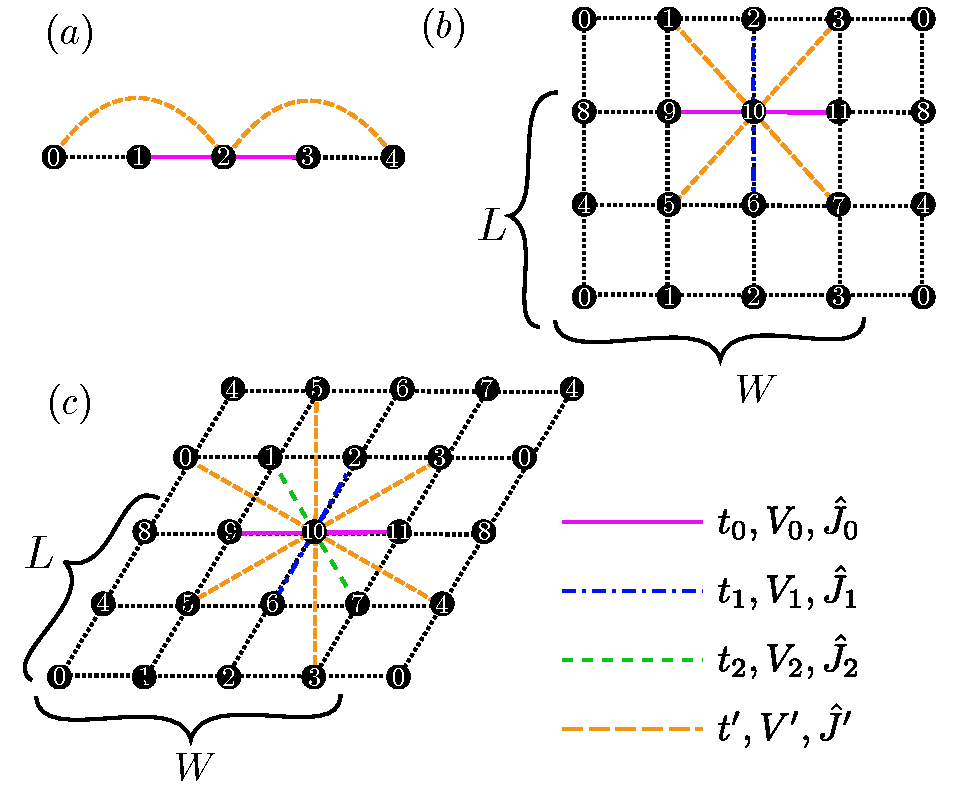
\includegraphics[width=10cm]{../figs/chap04_1_lattice.pdf}
    \caption{(a)1次元鎖、(b)2次元正方格子、(c)2次元三角格子の模式図. 
      ホッピング積分、オフサイトクーロン積分、スピン結合は、
      再近接サイト間(マゼンタの実線)ではそれぞれ$t,V,J$となり、
      次近接サイト間(緑の破線)ではそれぞれ$t',V',J'$となります。}
    \label{fig_chap04_1_lattice}
  \end{center}
\end{figure}

\begin{figure}[!htbp]
  \begin{center}
    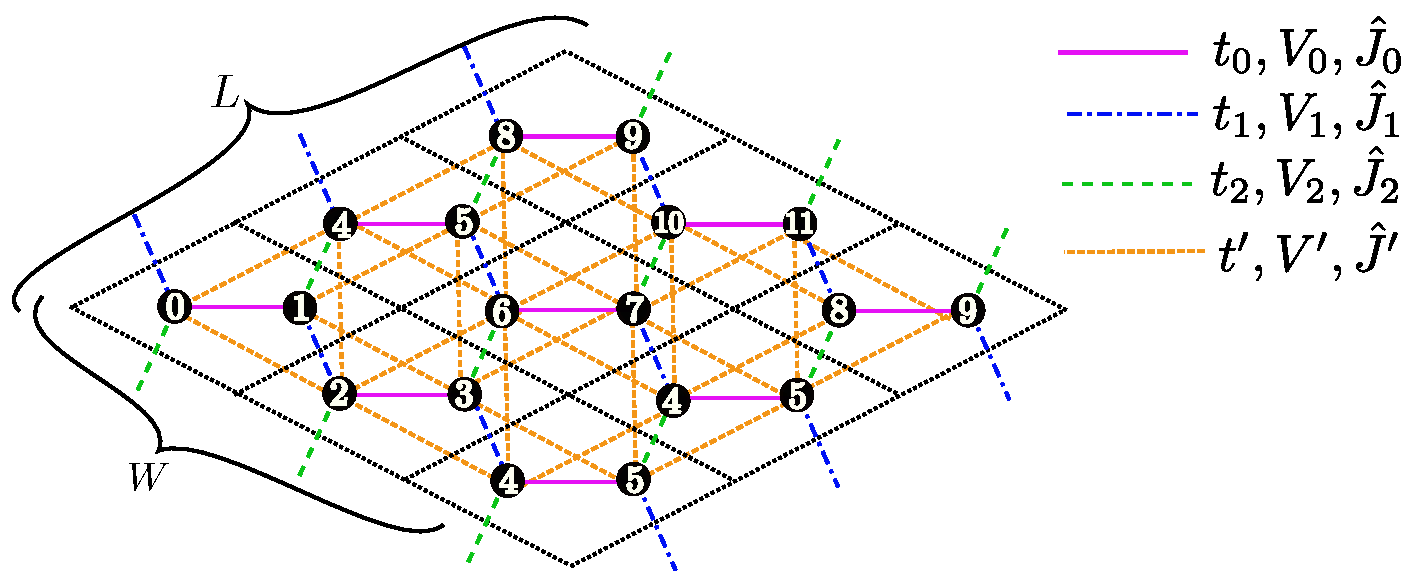
\includegraphics[width=15cm]{../figs/chap04_1_honeycomb.pdf}
    \caption{2次元異方的蜂の巣格子の模式図. 
      ホッピング積分、オフサイトクーロン積分、スピン結合は、
      ボンドの方向によって異なります。
      また、次近接のホッピング積分、オフサイトクーロン積分、スピン結合
      には対応していません。
    }
    \label{fig_chap04_1_honeycomb}
  \end{center}
\end{figure}

\begin{figure}[!htbp]
  \begin{center}
    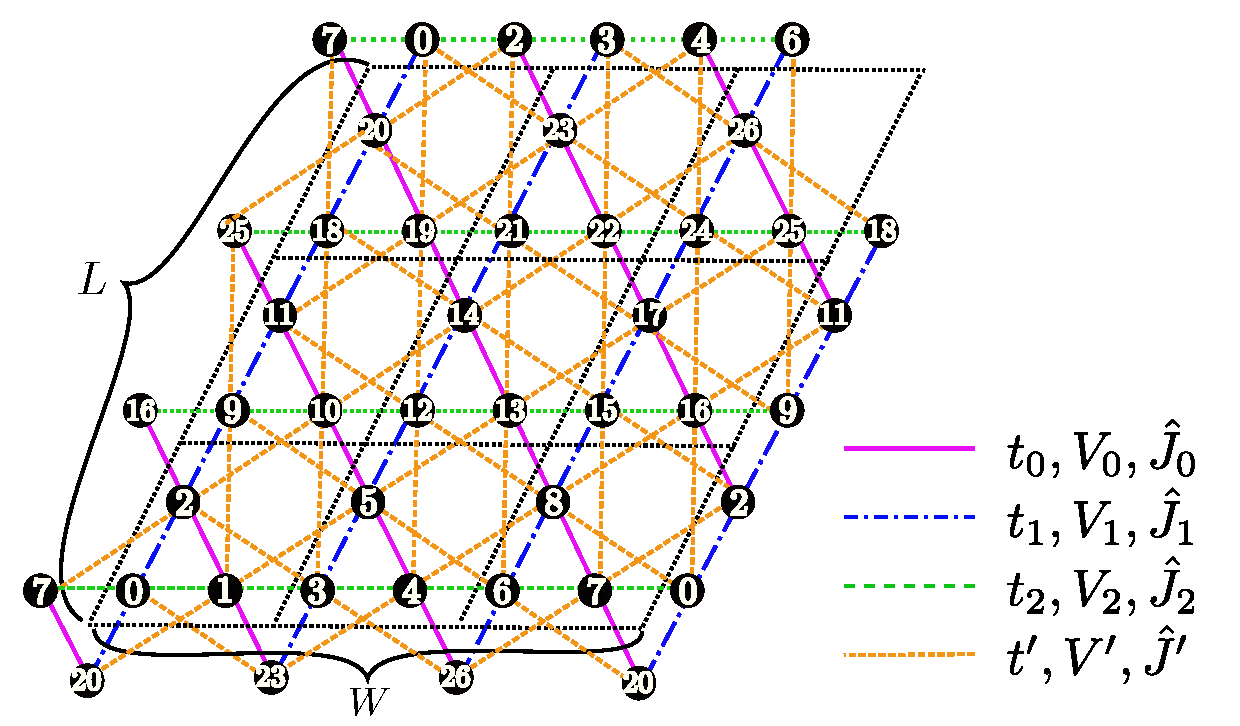
\includegraphics[width=15cm]{../figs/kagome.pdf}
    \caption{カゴメ格子の模式図. 
    }
    \label{fig_kagome}
  \end{center}
\end{figure}

\begin{figure}[!htbp]
  \begin{center}
    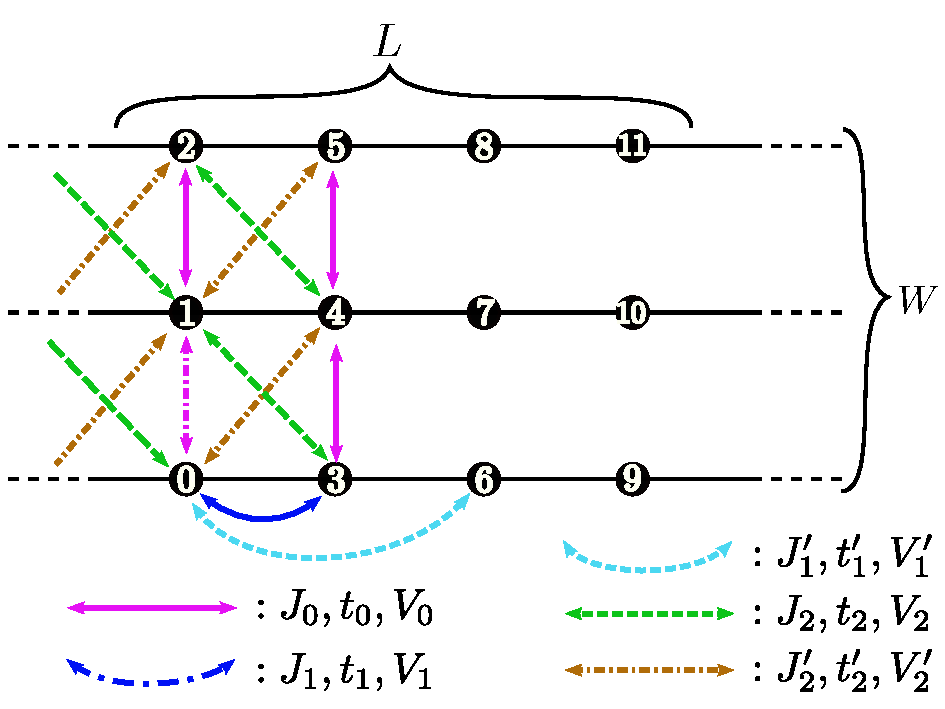
\includegraphics[width=10cm]{../figs/ladder.pdf}
    \caption{梯子格子の模式図. 
    }
    \label{fig_ladder}
  \end{center}
\end{figure}

\end{itemize}

\subsection{格子に関するパラメーター}

\subsubsection{1次元鎖[Fig. \ref{fig_chap04_1_lattice}(a)]}

\begin{itemize}

\item \verb|L|

{\bf 形式 :} 自然数

{\bf 説明 :} 鎖の長さを指定します. 

\end{itemize}

\subsubsection{梯子格子(Fig. \ref{fig_ladder})}

\begin{itemize}

\item \verb|L|

{\bf 形式 :} 自然数

{\bf 説明 :} 梯子の長さを指定します. 

\item \verb|W|

{\bf 形式 :} 自然数

{\bf 説明 :} 梯子の本数を指定します. 

\end{itemize}

\begin{figure}[!htbp]
  \begin{center}
    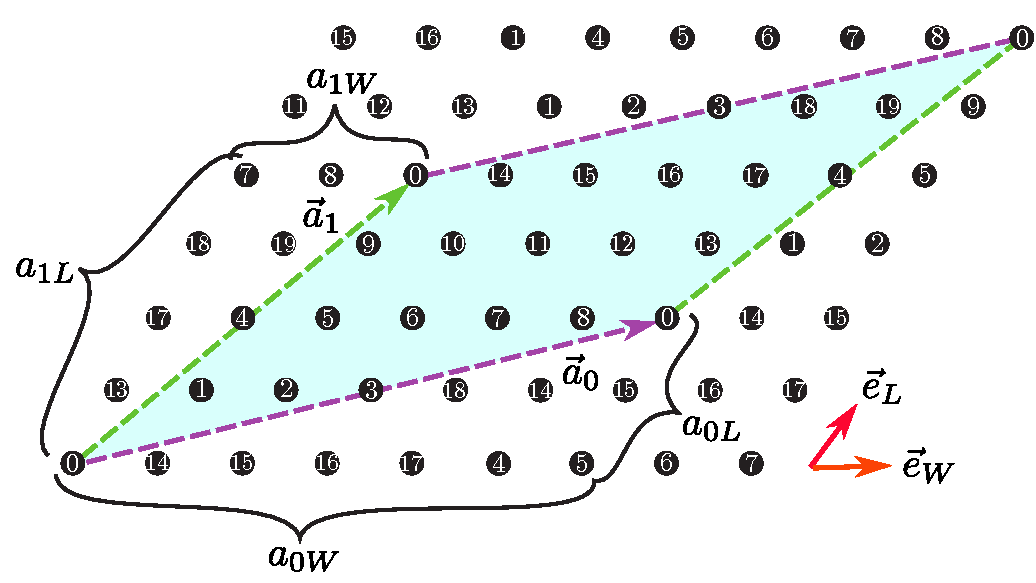
\includegraphics[width=15cm]{../figs/chap04_1_unitlattice.pdf}
    \caption{三角格子において、${\vec a}_0 = (6, 2), {\vec a}_1 = (2, 4)$とした場合のセル形状。
      ${\vec a}_0$(マゼンタ)および${\vec a}_1$(グリーン)
      で囲まれた部分(サイト数は20)が計算するセルとなる。
    }
    \label{fig_chap04_1_unitlattice}
  \end{center}
\end{figure}

\subsubsection{矩形格子[Fig. \ref{fig_chap04_1_lattice}(b)]、 
三角格子[Fig. \ref{fig_chap04_1_lattice}(c)]、
蜂の巣格子(Fig. \ref{fig_chap04_1_honeycomb})、
カゴメ格子(Fig. \ref{fig_kagome})}

これらの格子では、標準の単位胞(図中の黒の破線を参照)を用いて格子形状を指定する方法と、
それらとは別の方向に格子ベクトルを取る方法が選択できます。
また、両方を指定した場合にはプログラムを終了します。

\begin{itemize}

\item \verb|W|, \verb|L|

{\bf 形式 :} 自然数

{\bf 説明 :} 標準の単位胞の並び方を指定します。

\item \verb|a0W|, \verb|a0L|, \verb|a1W|, \verb|a1L|

{\bf 形式 :} 自然数

{\bf 説明 :} 格子を指定する2本のベクトル(${\vec a}_0, {\vec a}_1$)
を指定します (Fig. \ref{fig_chap04_1_unitlattice})。
これらのベクトルは標準の並進ベクトルを基底とした座標(Fractional coordinate)
で指定されます。

\end{itemize}

スタンダードモードで出力される\verb|lattice.gp|というファイルを使うと、
自分の意図した通りの格子のとり方になっているかどうかを確かめる事が出来ます。
このファイルは、次のようにして\verb|gnuplot|に読み込ませることが出来ます。
\begin{verbatim}
$ gnuplot lattice.gp
\end{verbatim}

\subsection{副格子}

以下パラメータを用いると変分波動関数のペア軌道部分に副格子の周期性を持たせることが出来ます。

\begin{itemize}

\item \verb|a0Wsub|, \verb|a0Lsub|, \verb|a1Wsub|, \verb|a1Lsub|, \verb|Wsub|, \verb|Lsub|

{\bf 形式 :} 自然数。デフォルトでは
\verb|a0Wsub=a0W|, \verb|a0Lsub=a0L|, \verb|a1Wsub=a1W|, \verb|a1Lsub=a1L|, 
\verb|Wsub=W|, \verb|Lsub=L|となる。
すなわち副格子を用いない。

{\bf 説明 :} これらのパラメーターの指定の仕方は
\verb|a0W|, \verb|a0L|, \verb|a1W|, \verb|a1L|, \verb|W|, \verb|L|
と同様です。
ただし、元の計算セルが副格子に整合しない場合にはプログラムを終了します。

\end{itemize}

%\subsection{保存量に関するパラメーター}
%
%\begin{itemize}
%\item \verb|nelec|
%
%{\bf 形式 :} 整数
%
%{\bf 説明 :} 全伝導電子数を指定します。
%\verb|model = "Fermion HubbardGC"|, \verb|"Spin"|, \verb|"SpinGC"|
%のときには指定しないでください。

%\item \verb|2Sz|

%{\bf 形式 :} 整数

%{\bf 説明 :} 全スピンのz 成分の2倍を指定します。
%\verb|model = "Fermion HubbardGC"|, \verb|SpinGC|
%のときには指定しないでください。
%\end{itemize}

\subsection{ハミルトニアンの各項の係数}

デフォルト値は特に記載されていないものについては0に設定してあります。
型が複素数のパラメータは「実部, 虚部」(間に``,'')の形式で指定し、
実数の場合には「実部」で指定が可能です。

\subsubsection{局所項}

\begin{itemize}

\item \verb|mu|

{\bf 形式 :} 実数

{\bf 説明 :} Hubbardおよび近藤格子模型での化学ポテンシャルを指定します。

\item \verb|U|

{\bf 形式 :} 実数

{\bf 説明 :} Hubbardおよび近藤格子模型でのオンサイトクーロン積分を指定します。

\item \verb|Jx|, \verb|Jy|, \verb|Jz|, \verb|Jxy|, 
  \verb|Jyx|, \verb|Jxz|, \verb|Jzx|, \verb|Jyz|, \verb|Jzy|

{\bf 形式 :} 実数

{\bf 説明 :} 近藤格子模型での、局在電子と遍歴電子のスピン結合を指定します。
また対角項について, \verb|Jx, Jy, Jz|を指定する代わりに、パラメータ\verb|J|を指定すると
\verb|Jx = Jy = Jz = J|が代入されます。
\verb|J|を指定した上で\verb|Jx|, \verb|Jy|, \verb|Jz|を指定した場合はプログラムを終了します。

\item \verb|h|, \verb|Gamma|, \verb|D|

{\bf 形式 :} 実数

{\bf 説明 :} スピン模型での縦磁場、横磁場、異方性パラメータを指定します。

\end{itemize}

下記の非局所項は、梯子格子の場合とそれ以外(1次元鎖、矩形格子、三角格子、蜂の巣格子、カゴメ格子)
の場合で指定の仕方が異なります。
また、各格子で指定可能なパラメーターをTable \ref{table_interactions}に表します。

\begin{table}[hbp]
  \begin{tabular}{|l||c|c|c|c|c|c|c|c|} \hline
    相互作用 & 1次元鎖 & 矩形格子 & 三角格子 & 蜂の巣格子 & カゴメ格子 & 梯子格子\\ 
    \hline \hline
     \verb|J|, \verb|t|, \verb|V|(省略形) & $\circ$	 & $\circ$ & $\circ$ & $\circ$ & $\circ$ & -\\ 
     \hline
    \verb|J'|, \verb|t'|, \verb|V'| & $\circ$	 & $\circ$	& $\circ$ 	& $\circ$ 	& $\circ$ & - \\ 
    \hline
    \verb|J0|, \verb|t0|, \verb|V0| & $\circ$  & $\circ$ 	& $\circ$ 	& $\circ$ 	& $\circ$ & $\circ$\\ 
    \hline
    \verb|J1|, \verb|t1|, \verb|V1| & -         	 & $\circ$ 	& $\circ$ 	& $\circ$ 	& $\circ$ & $\circ$\\ 
    \hline
    \verb|J2|, \verb|t2|, \verb|V2|  & -         	 & -    	& $\circ$ 	& $\circ$ 	& $\circ$ & $\circ$\\
    \hline
    \verb|J1'|, \verb|t1'|, \verb|V1'| & -		 &-	 	& -		& -		& -		& $\circ$\\
    \hline
    \verb|J2'| ,\verb|t2'|, \verb|V2'|  & -		 &-	 	& -		& -		& -		& $\circ$\\ 
    \hline
\end{tabular}
   \caption{各格子で定義可能な相互作用一覧。ただし、スピン結合については行列として与えることが可能。}
    \label{table_interactions}
\end{table}

\subsubsection{非局所項[梯子格子 (Fig. \ref{fig_ladder})]}

\begin{itemize}
\item \verb|t0|,  \verb|t1|,  \verb|t1'|,  \verb|t2|,  \verb|t2'|

{\bf 形式 :} 複素数

{\bf 説明 :} 梯子格子でのホッピング(Fig. \ref{fig_ladder}参照)を指定します。

\item \verb|V0|,  \verb|V1|,  \verb|V1'|,  \verb|V2|,  \verb|V2'|

{\bf 形式 :} 実数

{\bf 説明 :} 梯子格子でのオフサイトクーロン積分
(Fig. \ref{fig_ladder}参照)を指定します。

\item \verb|J0x|, \verb|J0y|, \verb|J0z|, \verb|J0xy|, 
  \verb|J0yx|, \verb|J0xz|, \verb|J0zx|, \verb|J0yz|, \verb|J0zy|
\item \verb|J1x|, \verb|J1y|, \verb|J1z|, \verb|J1xy|, 
  \verb|J1yx|, \verb|J1xz|, \verb|J1zx|, \verb|J1yz|, \verb|J1zy|
\item \verb|J1'x|, \verb|J1'y|, \verb|J1'z|, \verb|J1'xy|, 
  \verb|J1'yx|, \verb|J1'xz|, \verb|J1'zx|, \verb|J1'yz|, \verb|J1'zy|
\item \verb|J2x|, \verb|J2y|, \verb|J2z|, \verb|J2xy|, 
  \verb|J2yx|, \verb|J2xz|, \verb|J2zx|, \verb|J2yz|, \verb|J2zy|
\item \verb|J2'x|, \verb|J2'y|, \verb|J2'z|, \verb|J2'xy|, 
  \verb|J2'yx|, \verb|J2'xz|, \verb|J2'zx|, \verb|J2'yz|, \verb|J2'zy|

{\bf 形式 :} 実数

{\bf 説明 :} 梯子格子でのスピン相互作用
(Fig. \ref{fig_ladder}参照)を指定します。
また対角項について、例えば\verb|J0x, J0y, J0z|を指定する代わりに
パラメータ\verb|J0|を指定すると
\verb|J0x = J0y = J0z = J0|が代入されます。
\verb|J0|を指定した上で\verb|J0x, J0y, J0z|等も指定した場合はプログラムを終了します。
\verb|J1|, \verb|J1'|, \verb|J2|, \verb|J2'|についても同様です。

\end{itemize}

\subsubsection{非局所項 [梯子格子以外(Figs. \ref{fig_chap04_1_lattice}, \ref{fig_chap04_1_honeycomb},
\ref{fig_kagome})]}

\begin{itemize}
\item \verb|t0|,  \verb|t1|, \verb|t2|

{\bf 形式 :} 複素数

{\bf 説明 :} Hubbardおよび近藤格子模型での、最近接サイト間の各方向のホッピングを指定します。
Figs. \ref{fig_chap04_1_lattice}, \ref{fig_chap04_1_honeycomb},\ref{fig_kagome}
のそれぞれのボンド(異なる線種で表されています)
また、最近接ホッピングのボンド方向依存性(もしくは異方性)
がない場合は\verb|t0|,  \verb|t1|, \verb|t2|を
別々に指定する代わりにパラメータ\verb|t|を指定すると、\verb|t0 = t1 = t2 = t|が代入されます。
\verb|t|と\verb|t0|等の両方が指定された場合にはプログラムを終了します。

\item \verb|V0|,  \verb|V1|, \verb|V2|

{\bf 形式 :} 実数

{\bf 説明 :} Hubbardおよび近藤格子模型での、最近接サイト間のCoulomb積分を指定します。
また、サイト間Coulomb積分のボンド方向依存性がない場合は\verb|V0|,  \verb|V1|, \verb|V2|を
別々に指定する代わりにパラメータ\verb|V|を指定すると、\verb|V0 = V1 = V2 = V|が代入されます。
\verb|V|と\verb|V0|等の両方が指定された場合にはプログラムを終了します。

\item \verb|J0x|, \verb|J0y|, \verb|J0z|, \verb|J0xy|, 
  \verb|J0yx|, \verb|J0xz|, \verb|J0zx|, \verb|J0yz|, \verb|J0zy|
\item \verb|J1x|, \verb|J1y|, \verb|J1z|, \verb|J1xy|, 
  \verb|J1yx|, \verb|J1xz|, \verb|J1zx|, \verb|J1yz|, \verb|J1zy|
\item \verb|J2x|, \verb|J2y|, \verb|J2z|, \verb|J2xy|, 
  \verb|J2yx|, \verb|J2xz|, \verb|J2zx|, \verb|J2yz|, \verb|J2zy|

{\bf 形式 :} 実数

{\bf 説明 :} スピン模型での、最近接サイト間のスピン相互作用を指定します。
また対角項について、例えば\verb|J0x, J0y, J0z|を指定する代わりに
パラメータ\verb|J0|を指定すると
\verb|J0x = J0y = J0z = J0|が代入されます。
\verb|J0|を指定した上で\verb|J0x, J0y, J0z|等も指定した場合はプログラムを終了します。
\verb|J1|, \verb|J2|についても同様です。

スピン間相互作用のボンド方向依存性がない場合には、
\verb|Jx|, \verb|Jy|, \verb|Jz|, \verb|Jxy|, 
\verb|Jyx|, \verb|Jxz|, \verb|Jzx|, \verb|Jyz|, \verb|Jzy|
を指定すると、\verb|J0x = J1x = J2x = Jx|のようにすべてのボンド方向のスピン間相互作用に
同じ値を代入することが出来ます。
\verb|Jx|$\sim$\verb|Jzy|系列のどれかと\verb|J0x|$\sim$\verb|J2zy|系列のどれかを両方指定した
場合にはプログラムを終了します。
以下に最近接間スピン相互作用の指定方法の例を挙げます。

\begin{itemize}

\item ボンド方向依存性、スピン方向依存性、相互作用の非対角成分($J_{x y}$等)がない場合

\verb|J|を指定

\item ボンド方向依存性、相互作用の非対角成分がなく、スピン方向依存性がある場合

\verb|Jx, Jy, Jz|のうち\verb|0|でないものを指定

\item ボンド方向依存性がなく、スピン方向依存性、相互作用の非対角成分がある場合

\verb|Jx, Jy, Jz, Jxy, Jyz, Jxz, Jyx, Jzy, Jzx|のうち\verb|0|でないものを指定

\item スピン方向依存性、相互作用の非対角成分がなく、ボンド方向依存性がある場合

\verb|J0, J1, J2|のうち\verb|0|でないものを指定

\item スピン方向依存性がなく、ボンド方向依存性、相互作用の非対角成分がある場合

\verb|J0x, J0y, J0z, J1x, J1y, J1z, J2x, J2y, J2z|のうち\verb|0|でないものを指定

\item ボンド方向依存性、スピン方向依存性、相互作用の非対角成分がある場合

\verb|J0x|$\sim$\verb|J2zy|のすべてのうち\verb|0|でないものを指定

\end{itemize}
\item \verb|t'|

{\bf 形式 :} 複素数

{\bf 説明 :} Hubbardおよび近藤格子模型での、次近接サイト間の各方向のホッピングを指定します。

\item \verb|V'|

{\bf 形式 :} 実数

{\bf 説明 :} Hubbardおよび近藤格子模型での、次近接サイト間のCoulomb積分を指定します。

\item \verb|J'x|, \verb|J'y|, \verb|J'z|, \verb|J'xy|, 
  \verb|J'yx|, \verb|J'xz|, \verb|J'zx|, \verb|J'yz|, \verb|J'zy|

{\bf 形式 :} 実数

{\bf 説明 :} スピン模型での、次近接サイト間のスピン相互作用を指定します。
また対角項について、\verb|J'x, J'y, J'z|を指定する代わりに
パラメータ\verb|J'|を指定すると
\verb|J'x = J'y = J'z = J'|が代入されます。
\verb|J'|を指定した上で\verb|J'x, J'y, J'z|も指定した場合はプログラムを終了します。

\item \verb|phase0|, \verb|phase1|

  {\bf 形式 :} 複素数(デフォルトでは\verb|1.0|)
  
  {\bf 説明 :} 計算するセルの境界をまたいだホッピング項に付く位相因子を指定することが出来ます。
  $\vec{a}_0$方向、$\vec{a}_1$方向それぞれ別の位相因子を用いることが出来ます。
  1次元系では\verb|phase0|のみ使用できます。
  例えば、$i$サイトから$i+1$サイトへのホッピングで、
  正の方向に境界をまたいだ場合には次のようになります。
  \begin{align}
    ({\rm phase0}) \times t {\hat c}_{i+1 \sigma}^\dagger {\hat c}_{i \sigma}
    + ({\rm phase0})^* \times t^* {\hat c}_{i \sigma}^\dagger {\hat c}_{i+1 \sigma}
  \end{align}

\end{itemize}

\subsection{計算条件のパラメーター}

\begin{itemize}

\item \verb|OutputMode|

  {\bf 形式 :} \verb|"none"|, \verb|"correlation"|, \verb|"full"|のいずれか(デフォルトは\verb|correlation|)

  {\bf 説明 :} 計算を行う相関関数を指定します。
\verb|"none"|の場合は相関関数を計算しません。
\verb|"correlation"|を指定した場合には、1体部分はすべての$i, \sigma$について
$\langle c_{i \sigma}^{\dagger}c_{i \sigma} \rangle$を、
2体部分はすべての$i, j, \sigma, \sigma'$について
$\langle c_{i \sigma}^{\dagger}c_{i \sigma} c_{j \sigma'}^{\dagger}c_{j \sigma'} \rangle$
を計算します。
\verb|"full"|を指定した場合には、
1体部分はすべての$i, j, \sigma, \sigma'$について
$\langle c_{i \sigma}^{\dagger}c_{j \sigma'} \rangle$を、
2体部分はすべての$i_1, i_2, i_3, i_4, \sigma_1, \sigma_2, \sigma_3, \sigma_4$について
$\langle c_{i_1 \sigma_1}^{\dagger}c_{i_2 \sigma_2} c_{i_3 \sigma_3}^{\dagger}c_{i_4 \sigma_4} \rangle$
を計算します。
スピン系の演算子はBogoliubov表現により生成消滅演算子で表されています。
詳しくは\ref{sec_bogoliubov_rep}をご覧ください。

  \item  \verb|CDataFileHead|

 {\bf 形式 :} string型 (空白不可、必須)

{\bf 説明 :} アウトプットファイルのヘッダ。例えば、一体のGreen関数の出力ファイル名が{\bf xxx\_cisajs.dat}として出力されます(xxxに\verb|CDataFileHead|で指定した文字が記載)。

 \item  \verb|CParaFileHead|

 {\bf 形式 :} string型 (空白不可、必須)

{\bf 説明 :} 最適化された変分パラメータの出力ファイル名のヘッダ。最適化された変分パラメータが{\bf xxx\_opt.dat}ファイルとして出力されます(xxxに\verb|CParaFileHead|で指定した文字が記載)。
 
 
 \item  \verb|NVMCCalMode|

 {\bf 形式 :} int型 (\tr{デフォルト値 = 0})

{\bf 説明 :} [0] 変分パラメータの最適化、[1] 1 体・2 体のグリーン関数の計算。
 
 \item  \verb|NLanczosMode|

 {\bf 形式 :} int型 (\tr{デフォルト値 = 0})

{\bf 説明 :} [0] 何もしない、[1] Single Lanczos Step でエネルギーまで計算、
[2] Single Lanczos Step で1 体・2 体のグリーン関数まで計算
(条件: 1, 2 は\verb|NVMCCalMode| = 1のみ使用可能. 
また, pair hopping項, exchange 項がハミルトニアンに含まれる場合は使用できません)。
 
 \item  \verb|NDataIdxStart|

 {\bf 形式 :} int型 (\tr{デフォルト値 = 1})

{\bf 説明 :} 出力ファイルの付加番号。
\verb|NVMCCalMode|= 0 の場合は\verb|NDataIdxStart|が出力され、 
\verb|NVMCCalMode| = 1 の場合は、
\verb|NDataIdxStart|から連番で\verb|NDataQtySmp|個のファイルを出力します。
   
 \item  \verb|NDataQtySmp|

 {\bf 形式 :} int型 (\tr{デフォルト値 = 1})

{\bf 説明 :} 出力ファイルのセット数。 \verb|NVMCCalMode| = 1 の場合に使用します。

\item  \verb|nelec|

  {\bf 形式 :} {int型 (1以上、必須)}

  {\bf 説明 :} \tr{伝導電子の数。
    $\uparrow$電子と$\downarrow$電子の個数を足したものを入力してください。}

\item  \verb|NSPGaussLeg|

  {\bf 形式 :} {int型 (1以上、\tr{デフォルト値 = 8})}

  {\bf 説明 :} スピン量子数射影の$\beta$積分($S^y$回転)のGauss-Legendre求積法の分点数。


\item  \verb|NSPStot|

  {\bf 形式 :} int型 (0以上、\tr{デフォルト値 = 0})

  {\bf 説明 :}  スピン量子数。

\item  \verb|NMPTrans|

  {\bf 形式 :} int型 (1以上、\tr{デフォルト値は副格子内部の並進ベクトルの数})

  {\bf 説明 :} 
  運動量・格子対称性の量子数射影の個数。
  TransSymファイルで指定した重みで上から\verb|NMPTrans|個まで使用する。\tr{射影を行わない場合は1に設定する。}

 \item  \verb|NSROptItrStep|

{\bf 形式 :} int型 (1以上、\tr{デフォルト値 = 1000})

{\bf 説明 :} 
SR 法で最適化する場合の全ステップ数。\verb|NVMCCalMode|=0の場合のみ使用されます。
 
 \item  \verb|NSROptItrSmp|

{\bf 形式 :} int型 (1以上数、\tr{デフォルト値 = }\verb|NSROptItrStep|/10)

{\bf 説明 :} \verb|NSROptItrStep|ステップ中、最後の\verb|NSROptItrSmp|ステップでの各変分パラメータの平均値を最適値とする。\verb|NVMCCalMode|=0の場合のみ使用されます。

\item   \verb|DSROptRedCut|
   
{\bf 形式 :} double型 (\tr{デフォルト値 = 0.001})

{\bf 説明 :} SR 法安定化因子。手法論文の$\varepsilon_{\rm wf}$に対応。

 \item  \verb|DSROptStaDel| 
   
 {\bf 形式 :} double型 (\tr{デフォルト値 = 0.02})

  {\bf 説明 :} SR 法安定化因子。手法論文の$\varepsilon$に対応。
     
\item \verb|DSROptStepDt|

{\bf 形式 :} double型 (\tr{デフォルト値 = 0.02})

{\bf 説明 :} \tr{要確認(マニュアルに説明なし)}
 
\item \verb|NVMCWarmUp|

{\bf 形式 :} int型 (1以上、\tr{デフォルト値=10})

{\bf 説明 :}マルコフ連鎖の空回し回数。

\item \verb|NVMCIniterval|

{\bf 形式 :} int型 (1以上、\tr{デフォルト値=1})

{\bf 説明 :} サンプル間のステップ間隔。ローカル更新が\verb|Nsite|× \verb|NVMCIniterval| 回行わます。

\item \verb|NVMCSample|

{\bf 形式 :} int型 (1以上、\tr{デフォルト値=1000})

{\bf 説明 :} 期待値計算に使用するサンプル数。

\item \verb|RndSeed|

{\bf 形式 :} int型 

{\bf 説明 :} 乱数の初期seed。\tr{MPI 並列では各計算機に}\verb|RndSeed|\tr{+my rank+1 で初期seed が与えられます。}

 \item \verb|NSplitSize|

{\bf 形式 :} int型 (1以上、\tr{デフォルト値=1})

{\bf 説明 :} mpi内部並列を行う場合の並列数。

\item \verb|NStoreOO|

{\bf 形式 :} int型 (1以上、\tr{デフォルト値=0})

{\bf 説明 :} 期待値$\langle O_k O_l \rangle$を計算するとき行列-行列積にするオプション(1で機能On)。
 
\item  \verb|ComplexType|
  
  {\bf 形式 :} int型 (\verb|0|もしくは\verb|1|、デフォルト値\verb|0|)

  {\bf 説明 :} \verb|0|のとき変分パラメータの実部のみを、\verb|1|のとき実部/虚部両方を最適化します。

\end{itemize}


\newpage
\section{詳細入力ファイル}
\label{Ch:HowToExpert}

\tr{ここではmVMCで使用する詳細入力ファイル(*def)のフォーマットに関して説明します。
入力ファイルの種別は以下の6つで分類されます。なお、キーワードの後にある括弧内に記載されているファイル名はvmcdry.outにより作成されるファイル名を表します。}
\begin{description}
\item[(1)~List:]
~\\{\bf キーワード指定なし (namelist.def)}:
使用するinput fileの名前のリストを書きます。なお、ファイル名は任意に指定することができます。
\item[(2)~Basic parameters:]
~\\{\bf ModPara (modpara.def)}: 計算時に必要な基本的なパラメーター(サイトの数、電子数など)を設定します。
~\\{\bf LocSpin (locspn.def)}: 局在スピンの位置を設定します。
\item[\tr{(3)~Set Hamiltonian:}] 
~\\電子系の表式で記載されるハミルトニアン
\begin{equation}
{\cal H}={\cal H}_T+{\cal H}_U+{\cal H}_V+{\cal H}_H+{\cal H}_E+{\cal H}_P+{\cal H}_I
\end{equation}
を指定します。各ハミルトニアンのパラメータは以下のファイルで指定します。
~\\{\bf Trans (trans.def)}: 
${\cal H}_T=\tr{-}\sum_{i, j}\sum_{\sigma_1, \sigma2}t_{ij\sigma_1\sigma_2} c_{i\sigma_1}^{\dag}c_{j\sigma_2}$
で表される一体項のハミルトニアンに対して$t_{ij\sigma_1\sigma_2}$を指定します。\\
~\\{\bf CoulombIntra (coulombintra.def)}: 
${\cal H}_U=\sum_{i} U_i n_ {i \uparrow}n_{i \downarrow}$で表される相互作用に対して$U_i$を指定します($n_{i \sigma}=c_{i\sigma}^{\dag}c_{i\sigma}$)。\\
~\\{\bf CoulombInter (coulombinter.def)}: 
${\cal H}_V=\sum_{i,j} V_{ij}n_ {i}n_{j}$で表される相互作用に対して$V_{ij}$を指定します($n_i=n_{i\uparrow}+n_{i\downarrow}$)。\\
~\\{\bf Hund (hund.def)}: 
${\cal H}_H=\tr{-}\sum_{i,j}J_{ij}^{\rm Hund} (n_{i\uparrow}n_{j\uparrow}+n_{i\downarrow}n_{j\downarrow})$
で表される相互作用に対して$J_{ij}^{\rm Hund}$を指定します。\\
~\\{\bf Exchange (exchange.def)}:
${\cal H}_E=\sum_{i,j}J_{ij}^{\rm Ex} (c_ {i \uparrow}^{\dag}c_{j\uparrow}c_{j \downarrow}^{\dag}c_{i  \downarrow}+c_ {i \downarrow}^{\dag}c_{j\downarrow}c_{j \uparrow}^{\dag}c_{i  \uparrow})$
で表される相互作用に対して$J_{ij}^{\rm Ex}$を指定します。\\
~\\{\bf PairHop}:  ${\cal H}_P =\sum_{i,j}J_{ij}^{\rm Pair} c_ {i \uparrow}^{\dag}c_{j\uparrow}c_{i \downarrow}^{\dag}c_{j  \downarrow}
$で表される相互作用に対して$J_{ij}^{\rm Pair}$を指定します。
~\\{\bf InterAll}: ${\cal H}_I=\sum_{i,j,k,l}\sum_{\sigma_1,\sigma_2, \sigma_3, \sigma_4}
I_{ijkl\sigma_1\sigma_2\sigma_3\sigma_4}c_{i\sigma_1}^{\dagger}c_{j\sigma_2}c_{k\sigma_3}^{\dagger}c_{l\sigma_4}$で表される一般二体相互作用に対して$I_{ijkl\sigma_1\sigma_2\sigma_3\sigma_4}$を指定します。\\
\item[(4)~Set condition of variational parameters:] 
~\\ \tr{最適化する変分パラメータを指定します}。変分波動関数は
\begin{equation}
|\psi \rangle = {\cal P}_G{\cal P}_J{\cal P}_{d-h}^{(2)}{\cal P}_{d-h}^{(4)}{\cal L}^S{\cal L}^K{\cal L}^P |\phi_{\rm pair} \rangle,
\end{equation}
で与えられます。ここで、一体部分は実空間のペア関数
\begin{equation}
|\phi_{\rm pair} \rangle = \left[\sum_{i, j=1}^{N_s} f_{ij}c_{i\uparrow}^{\dag}c_{j\downarrow}^{\dag} \right]^{N/2}|0 \rangle,
\end{equation}
を用いた波動関数で表されます。ここで$N$は全電子数、$N_s$は全サイト数です。
最適化する変分パラメータは以下のファイルを用いて指定します。
~\\{\bf Gutzwiller (gutzwilleridx.def)}: ${\cal P}_G=\exp\left[ \sum_i g_i n_{i\uparrow} n_{i\downarrow} \right]$のうち、最適化の対象とする変分パラメータ$g_i$を指定します。
~\\{\bf Jastrow (jastrowidx.def)}: ${\cal P}_J=\exp\left[\frac{1}{2} \sum_{i\neq j} v_{ij} n_i n_j\right]$のうち、最適化の対象とする変分パラメータ$v_{ij}$を指定します。
~\\{\bf DH2}:  ${\cal P}_{d-h}^{(2)}= \exp \left[ \sum_t \sum_{n=0}^2 (\alpha_{2nt}^d \sum_{i}\xi_{i2nt}^d+\alpha_{2nt}^h \sum_{i}\xi_{i2nt}^h)\right]$で表される2サイトのdoublon-holon相関因子を指定します。相関因子に関する詳細は文献\cite{Tahara2008}を参照してください。
~\\{\bf DH4}:  ${\cal P}_{d-h}^{(4)}= \exp \left[ \sum_t \sum_{n=0}^4 (\alpha_{4nt}^d \sum_{i}\xi_{i4nt}^d+\alpha_{4nt}^h \sum_{i}\xi_{i4nt}^h)\right]$で表される4サイトのdoublon-holon相関因子を指定します。相関因子に関する詳細は文献\cite{Tahara2008}の説明を参照してください。
~\\{\bf Orbital (orbitalidx.def)}: ペア軌道$|\phi_{\rm pair} \rangle = \left[\sum_{i, j=1}^{N_s} f_{ij}c_{i\uparrow}^{\dag}c_{j\downarrow}^{\dag} \right]^{N/2}|0 \rangle$を設定します。
~\\{\bf TransSym (qptransidx.def)}: 運動量射影${\cal L}_K=\frac{1}{N_s}\sum_{{\bm R}}e^{i {\bm K} \cdot{\bm R} } \hat{T}_{\bm R}$と格子対称性射影${\cal L}_P=\sum_{\alpha}p_{\alpha} \hat{G}_{\alpha}$に関する指定を行います。ここで、${\bm K}$は全運動量、$\hat{T}_{\bm R}$は並進ベクトル${\bm R}$に対応する並進演算子、$\hat{G}_{\alpha}$は格子の点群演算子、$p_\alpha$はパリティをそれぞれ表します。

\item[(5)~Initial variational parameters:]
~\\ 変分パラメータに関する初期値を与えます。キーワード指定されない場合には$0$が初期値として設定されます。
~\\{\bf InGutzwiller}: ${\cal P}_G=\exp\left[ \sum_i g_i n_{i\uparrow} n_{i\downarrow} \right]$のうち、変分パラメータ$g_i$の初期値を指定します。
~\\{\bf InJastrow}: ${\cal P}_J=\exp\left[\frac{1}{2} \sum_{i\neq j} v_{ij} n_i n_j\right]$のうち、変分パラメータ$v_{ij}$の初期値を指定します。
~\\{\bf InDH2}:  ${\cal P}_{d-h}^{(2)}= \exp \left[ \sum_t \sum_{n=0}^2 (\alpha_{2nt}^d \sum_{i}\xi_{i2nt}^d+\alpha_{2nt}^h \sum_{i}\xi_{i2nt}^h)\right]$で表される2サイトのdoublon-holon相関因子$\alpha_{2nt}^{d(h)}$の初期値を指定します。
~\\{\bf InDH4}:  ${\cal P}_{d-h}^{(4)}= \exp \left[ \sum_t \sum_{n=0}^4 (\alpha_{4nt}^d \sum_{i}\xi_{i4nt}^d+\alpha_{4nt}^h \sum_{i}\xi_{i4nt}^h)\right]$で表される4サイトのdoublon-holon相関因子$\alpha_{4nt}^{d(h)}$の初期値を指定します。
~\\{\bf InOrbital}: ペア軌道$|\phi_{\rm pair} \rangle = \left[\sum_{i, j=1}^{N_s} f_{ij}c_{i\uparrow}^{\dag}c_{j\downarrow}^{\dag} \right]^{N/2}|0 \rangle$の$ f_{ij}$に関する初期値を設定します。


\item[(6)~Output:]
~\\{\bf OneBodyG (greenone.def)}:出力する一体Green関数を指定します。
 $\langle c^{\dagger}_{i\sigma_1}c_{j\sigma_2}\rangle$が出力されます。

 {\bf TwoBodyG (greentwo.def)}:出力する二体Green関数を指定します。
 $\langle c^{\dagger}_{i\sigma_1}c_{j\sigma_2}c^{\dagger}_{k \sigma_3}c_{l\sigma_4}\rangle$
が出力されます。
\end{description}
%%%%%%%%%%%%%%%%%%%%%%
\newpage
~\subsection{入力ファイル指定用ファイル}
\label{Subsec:InputFileList}
計算で使用する入力ファイル一式を指定します。ファイル形式に関しては、以下のようなフォーマットをしています。\\
\begin{minipage}{10cm}
\begin{screen}
\begin{verbatim}
ModPara  modpara.def
LocSpin  zlocspn.def
Trans    ztransfer.def
InterAll zinterall.def
Orbital orbitalidx.def
OneBodyG zcisajs.def
TwoBodyG	zcisajscktaltdc.def
\end{verbatim}
\end{screen}
\end{minipage}
\\
\subsubsection{ファイル形式}
[string01]~[string02]
\subsubsection{パラメータ}
 \begin{itemize}
   \item  $[$string01$]$
   
   {\bf 形式 :} string型 (固定)
   
   {\bf 説明 :} キーワードを指定します。
   
   \item  $[$string02$]$
   
    {\bf 形式 :} string型 

   {\bf 説明 :} キーワードにひも付けられるファイル名を指定します(任意)。
 \end{itemize}
\subsubsection{使用ルール}
本ファイルを使用するにあたってのルールは以下の通りです。
\begin{itemize}
\item キーワードを記載後、半角空白(複数可)を開けた後にファイル名を書きます。ファイル名は自由に設定できます。
\item ファイル読込用キーワードはTable\ref{Table:Defs}により指定します。
\item 必ず指定しなければいけないキーワードはModPara, LocSpin, Orbitalです。それ以外のキーワードについては、指定がない場合はデフォルト値が採用されます(変分パラメータについては最適化されず、固定する設定となります)。詳細は各ファイルの説明を参照してください。
\item 各キーワードは順不同に記述できます。
\item 指定したキーワード、ファイルが存在しない場合はエラー終了します。
\item $\#$で始まる行は読み飛ばされます。
\end{itemize}

 \begin{table*}[h!]
\begin{center}
  \begin{tabular}{|ll|} \hline
           Keywords     & 対応するファイルの概要       \\   \hline\hline
           ModPara$^*$       &  計算用のパラメータを指定       \\ \hline 
           %%%%%%%%%%%%%%%%%%  
           LocSpin$^*$         &  局在・遍歴スピンを指定       \\ 
           Trans       &   一般的な一体相互作用を指定  \\
           InterAll  &   一般的な二体相互作用を指定 \\  
           CoulombIntra  &   CoulombIntra interactions. \\  
           CoulombInter  &   CoulombInter  interactions. \\  
           Hund  &   Hund couplings. \\  
           PairHop  &  Pair hopping couplings. \\  
           Exchange  &  Exchange couplings. \\  \hline
           %%%%%%%%%%%%%%%%%%
           Gutzwiller & Gutzwiller factors.\\
           Jastrow & Charge Jastrow factors.\\
           DH2 & 2-site doublon-holon correlation factors.\\
           DH4 & 4-site doublon-holon correlation factors.\\
           Orbital$^*$  & Pair orbital factors.\\
           TransSym$^*$  & Translational and lattice symmetry operation. \\ \hline
           %%%%%%%%%%%%%%%%%%
           InGutzwiller & Initial values of Gutzwiller factors.\\
           InJastrow & Initial values of charge Jastrow factors.\\
           InDH2 & Initial values of 2-site doublon-holon correlation factors.\\
           InDH4 & Initial values of 4-site doublon-holon correlation factors.\\
           InOrbital & Initial values of pair orbital factors.\\ \hline
           %%%%%%%%%%%%%%%%%%
           OneBodyG         &   Output components for Green functions $\langle c_{i\sigma}^{\dagger}c_{j\sigma}\rangle$           \\   
           TwoBodyG &   Output components for Correlation functions $\langle c_{i\sigma}^{\dagger}c_{j\sigma}c_{k\tau}^{\dagger}c_{l\tau}\rangle$  \\   \hline
  \end{tabular}
\end{center}
\caption{List of the definition files. * が付いているファイルは実行時に必ず必要となります。}
\label{Table:Defs}
\end{table*}%

\newpage
%----------------------------------
\subsection{ModParaファイル}
\label{Subsec:modpara}
計算で使用するパラメータを指定します。以下のようなフォーマットをしています。\\
\begin{minipage}{10cm}
\begin{screen}
\begin{verbatim}
--------------------
Model_Parameters   0
--------------------
VMC_Cal_Parameters
--------------------
CDataFileHead  zvo
CParaFileHead  zqp
--------------------
NVMCCalMode    0
NLanczosMode   0
--------------------
NDataIdxStart  1
NDataQtySmp    1
--------------------
Nsite          16
Nelectron      8
NSPGaussLeg    1
NSPStot        0
NMPTrans       1
NSROptItrStep  1200
NSROptItrSmp   100
DSROptRedCut   0.001
DSROptStaDel   0.02
DSROptStepDt   0.02
NVMCWarmUp     10
NVMCIniterval  1
NVMCSample     1000
NExUpdatePath  0
RndSeed        11272
NSplitSize     1
NStore         1  
\end{verbatim}
\end{screen}
\end{minipage}

\subsubsection{ファイル形式}
以下のように行数に応じ異なる形式をとります。
 \begin{itemize}
   \item  1 - 5行:  ヘッダ(何が書かれても問題ありません)。
   \item  6行:  [string01]~[string02]
   \item  7 - 8行: ヘッダ(何が書かれても問題ありません)
   \item  9行以降: [string01]~[int01]
  \end{itemize}
各項目の対応関係は以下の通りです。
\begin{itemize}
   \item  $[$string01$]$
   
   {\bf 形式 :} string型 (固定)

  {\bf 説明 :} キーワードの指定を行います。
   
   \item  $[$string02$]$
   
   {\bf 形式 :} string型 (空白不可)

  {\bf 説明 :} アウトプットファイルのヘッダを指定します。

   \item  $[$int01$]$
   
   {\bf 形式 :} int型 (空白不可)

  {\bf 説明 :} キーワードでひも付けられるパラメータを指定します。

  \end{itemize}

\subsubsection{使用ルール}
本ファイルを使用するにあたってのルールは以下の通りです。
\begin{itemize}
\item 9行目以降ではキーワードを記載後、半角空白(複数可)を開けた後に整数値を書きます。
\item 行数固定で読み込みを行う為、パラメータの省略はできません。
\end{itemize}

~\subsubsection{キーワード}
 \begin{itemize}
  \item  \verb|CDataFileHead|

 {\bf 形式 :} string型 (空白不可、必須)

{\bf 説明 :} アウトプットファイルのヘッダ。例えば、一体のGreen関数の出力ファイル名が{\bf xxx\_cisajs.dat}として出力されます(xxxに\verb|CDataFileHead|で指定した文字が記載)。

 \item  \verb|CParaFileHead|

 {\bf 形式 :} string型 (空白不可、必須)

{\bf 説明 :} 最適化された変分パラメータの出力ファイル名のヘッダ。最適化された変分パラメータが{\bf xxx\_opt.dat}ファイルとして出力されます(xxxに\verb|CParaFileHead|で指定した文字が記載)。
 
 
 \item  \verb|NVMCCalMode|

 {\bf 形式 :} int型 (デフォルト値 = 0)

{\bf 説明 :} [0] 変分パラメータの最適化、[1] 1 体・2 体のグリーン関数の計算。
 
 \item  \verb|NLanczosMode|

 {\bf 形式 :} int型 (デフォルト値 = 0)

{\bf 説明 :} [0] 何もしない、[1] Single Lanczos Step でエネルギーまで計算、[2] Single Lanczos Step で1 体・2 体のグリーン関数まで計算(条件: 1, 2 は\verb|NVMCCalMode| = 1のみ使用可能. また, pair hopping項, exchange 項がハミルトニアンに含まれる場合は使用できません)。
 
 \item  \verb|NDataIdxStart|

 {\bf 形式 :} int型 (デフォルト値 = 0)

{\bf 説明 :} 出力ファイルの付加番号。\verb|NVMCCalMode|= 0 の場合は\verb|NDataIdxStart|が出力され、 \verb|NVMCCalMode| = 1 の場合は、\verb|NDataIdxStart|から連番で\verb|NDataQtySmp|個のファイルを出力します。
   
 \item  \verb|NDataQtySmp|

 {\bf 形式 :} int型 (デフォルト値 = 1)

{\bf 説明 :} 出力ファイルのセット数。 \verb|NVMCCalMode| = 1 の場合に使用します。

 \item  \verb|Nsite|

{\bf 形式 :} int型 (1以上、必須)

{\bf 説明 :} サイト数を指定する整数。  

\item  \verb|Nelectron|

{\bf 形式 :} {int型 (1以上、必須)}

{\bf 説明 :} \tr{$\uparrow$電子の個数。$S_z=0$部分空間で計算するので、$\uparrow$電子と$\downarrow$電子の個数は等しい。}

 \item  \verb|NSPGaussLeg|

{\bf 形式 :} {int型 (1以上、デフォルト値 = 1)}

{\bf 説明 :} スピン量子数射影の$\beta$積分($S^y$回転)のGauss-Legendre求積法の分点数。

 \item  \verb|NSPStot|

{\bf 形式 :} int型 (0以上、デフォルト値 = 0)

{\bf 説明 :}  スピン量子数。

 \item  \verb|NMPTrans|

{\bf 形式 :} int型 (1以上、デフォルト値 = 1)

{\bf 説明 :} 
運動量・格子対称性の量子数射影の個数。TransSymファイルで指定した重みで上から\verb|NMPTrans|個まで使用する。\tr{射影を行わない場合は1に設定する。}

 \item  \verb|NSROptItrStep|

{\bf 形式 :} int型 (1以上、デフォルト値 = 1000)

{\bf 説明 :} 
SR 法で最適化する場合の全ステップ数。\verb|NVMCCalMode|=0の場合のみ使用されます。
 
 \item  \verb|NSROptItrSmp|

{\bf 形式 :} int型 (1以上数、デフォルト値 = \verb|NSROptItrStep|/10)

{\bf 説明 :} \verb|NSROptItrStep|ステップ中、最後の\verb|NSROptItrSmp|ステップでの各変分パラメータの平均値を最適値とする。\verb|NVMCCalMode|=0の場合のみ使用されます。

\item   \verb|DSROptRedCut|
   
{\bf 形式 :} double型 (デフォルト値 = 0.001)

{\bf 説明 :} SR 法安定化因子。手法論文\cite{Tahara2008}の$\varepsilon_{\rm wf}$に対応。

 \item  \verb|DSROptStaDel| 
   
 {\bf 形式 :} double型 (デフォルト値 = 0.02)

  {\bf 説明 :} SR 法安定化因子。手法論文\cite{Tahara2008}の$\varepsilon$に対応。
     
\item \verb|DSROptStepDt|

{\bf 形式 :} double型 

{\bf 説明 :} \tr{要確認(マニュアルに説明なし)}
 
\item \verb|NVMCWarmUp|

{\bf 形式 :} int型 (1以上、\tr{デフォルト値=10})

{\bf 説明 :}マルコフ連鎖の空回し回数。

\item \verb|NVMCIniterval|

{\bf 形式 :} int型 (1以上、\tr{デフォルト値=1})

{\bf 説明 :} サンプル間のステップ間隔。ローカル更新が\verb|Nsite|× \verb|NVMCIniterval| 回行わます。

\item \verb|NVMCSample|

{\bf 形式 :} int型 (1以上、\tr{デフォルト値=1000})

{\bf 説明 :} 期待値計算に使用するサンプル数。

\item \verb|NExUpdatePath|

{\bf 形式 :} int型 (1以上)

{\bf 説明 :} ローカル更新で2 電子交換を[0] 認めない、[1] 認める。\tr{デフォルト設定は局在スピンが一つでもある場合は1、それ以外は0となります}。

\item \verb|RndSeed|

{\bf 形式 :} int型 

{\bf 説明 :} 乱数の初期seed。\tr{MPI 並列では各計算機に}\verb|RndSeed|\tr{+my rank+1 で初期seed が与えられます。}

 \item \verb|NSplitSize|

{\bf 形式 :} int型 (1以上、\tr{デフォルト値=1})

{\bf 説明 :} mpi内部並列を行う場合の並列数。

\item \verb|NStore|

{\bf 形式 :} int型 (1以上、\tr{デフォルト値=1})

{\bf 説明 :} 期待値$\langle O_k O_l \rangle$を計算するとき行列-行列積にして高速化するオプション(1で機能On、\tr{モンテカルロサンプリング数に応じてメモリの消費が増大します})。
 
 \end{itemize}


\newpage
%----------------------------------
\subsection{LocSpin指定ファイル}
\label{Subsec:locspn}
局在スピンを指定します。以下のようなフォーマットをしています。\\
\begin{minipage}{10cm}
\begin{screen}
\begin{verbatim}
================================ 
NlocalSpin     6  
================================ 
========i_0LocSpn_1IteElc ====== 
================================ 
    0      1
    1      0
    2      1
    3      0
    4      1
    5      0
    6      1
    7      0
    8      1
    9      0
   10      1
   11      0
\end{verbatim}
\end{screen}
\end{minipage}


\subsubsection{ファイル形式}
以下のように行数に応じ異なる形式をとります。
 \begin{itemize}
   \item  1行:  ヘッダ(何が書かれても問題ありません)。
   \item  2行:   [string01]~[int01]
   \item  3-5行:  ヘッダ(何が書かれても問題ありません)。
   \item  6行以降:  [int02]~[int03]
  \end{itemize}
 \subsubsection{パラメータ}
 \begin{itemize}

 \item  $[$string01$]$

 {\bf 形式 :} string型 (空白不可)

{\bf 説明 :} 局在スピンの総数を示すキーワード(任意)。


  \item  $[$int01$]$

 {\bf 形式 :} int型 (空白不可)

{\bf 説明 :} 局在スピンの総数を指定する整数。

 
  \item  $[$int02$]$

 {\bf 形式 :} int型 (空白不可)

{\bf 説明 :} サイト番号を指定する整数。0以上\verb|Nsite|{未満}で指定します。

 
  \item  $[$int03$]$

 {\bf 形式 :} int型 (空白不可)

{\bf 説明 :} 局在スピンか遍歴電子かを指定する整数。\\
{
0: 遍歴電子\\
$n>0$: $2S=n$の局在スピン\\
}
を選択することが出来ます。
 \end{itemize}

\subsubsection{使用ルール}
本ファイルを使用するにあたってのルールは以下の通りです。
\begin{itemize}
\item 行数固定で読み込みを行う為、ヘッダの省略はできません。
\item $[$int01$]$と$[$int03$]$で指定される局在電子数の総数が異なる場合はエラー終了します。
\item $[$int02$]$の総数が全サイト数と異なる場合はエラー終了します。
\item $[$int02$]$が全サイト数以上もしくは負の値をとる場合はエラー終了します。
\end{itemize}


\newpage
\subsection{Trans指定ファイル}
\label{Subsec:Trans}
ここではハミルトニアン
\begin{align}
H +=-\sum_{ij\sigma_1\sigma2} t_{ij\sigma_1\sigma2}c_{i\sigma_1}^{\dag}c_{j\sigma_2}
\end{align}
に対するTransfer積分$t_{ij\sigma_1\sigma2}$を指定します。以下にファイル名を記載します。\\
\begin{minipage}{12.5cm}
\begin{screen}
\begin{verbatim}
======================== 
NTransfer      24  
======================== 
========i_j_s_tijs====== 
======================== 
    0     0     2     0   1.000000  0.000000
    2     0     0     0   1.000000  0.000000
    0     1     2     1   1.000000  0.000000
    2     1     0     1   1.000000  0.000000
    2     0     4     0   1.000000  0.000000
    4     0     2     0   1.000000  0.000000
    2     1     4     1   1.000000  0.000000
    4     1     2     1   1.000000  0.000000
    4     0     6     0   1.000000  0.000000
    6     0     4     0   1.000000  0.000000
    4     1     6     1   1.000000  0.000000
    6     1     4     1   1.000000  0.000000
    6     0     8     0   1.000000  0.000000
    8     0     6     0   1.000000  0.000000
…
\end{verbatim}
\end{screen}
\end{minipage}

\subsubsection{ファイル形式}
以下のように行数に応じ異なる形式をとります。
 \begin{itemize}
   \item  1行:  ヘッダ(何が書かれても問題ありません)。
   \item  2行:   [string01]~[int01]
   \item  3-5行:  ヘッダ(何が書かれても問題ありません)。
   \item  6行以降: [int02]~~[int03]~~[int04]~~[int05]~~[double01]~~[double02] 
  \end{itemize}
\subsubsection{パラメータ}
 \begin{itemize}

   \item  $[$string01$]$
   
    {\bf 形式 :} string型 (空白不可)

   {\bf 説明 :} Transfer総数のキーワード名を指定します(任意)。

   \item  $[$int01$]$
   
    {\bf 形式 :} int型 (空白不可)

   {\bf 説明 :} Transferの総数を指定します。

  \item  $[$int02$]$, $[$int04$]$

 {\bf 形式 :} int型 (空白不可)

{\bf 説明 :} サイト番号を指定する整数。0以上\verb|Nsite|{未満}で指定します。
 
  \item  $[$int03$]$, $[$int05$]$

 {\bf 形式 :} int型 (空白不可)

{\bf 説明 :} スピンを指定する整数。\\
0: アップスピン\\
1: ダウンスピン\\
を選択することが出来ます。


 \item  $[$double01$]$
   
   {\bf 形式 :} double型 (空白不可)

  {\bf 説明 :}  $t_{ij\sigma_1\sigma_2}$の実部を指定します。

 \item  $[$double02$]$
   
   {\bf 形式 :} double型 (空白不可)

  {\bf 説明 :}  $t_{ij\sigma_1\sigma_2}$の虚部を指定します。
\end{itemize}

\subsubsection{使用ルール}
本ファイルを使用するにあたってのルールは以下の通りです。
\begin{itemize}
\item 行数固定で読み込みを行う為、ヘッダの省略はできません。
\item Hamiltonianがエルミートという制限から$t_{ij\sigma_1\sigma_2}=t_{ji\sigma_2\sigma_1}^{\dagger}$の関係を満たす必要があります。上記の関係が成立しない場合にはエラー終了します。
\item 成分が重複して指定された場合にはエラー終了します。
\item $[$int01$]$と定義されているTrasferの総数が異なる場合はエラー終了します。
\item $[$int02$]$-$[$int05$]$を指定する際、範囲外の整数を指定した場合はエラー終了します。
\end{itemize}

\newpage
\subsection{InterAll指定ファイル}
\label{Subsec:interall}
ここでは一般二体相互作用をハミルトニアンに付け加えます。付け加える項は以下で与えられます。
\begin{equation}
H+=\sum_{i,j,k,l}\sum_{\sigma_1,\sigma_2, \sigma_3, \sigma_4}
I_{ijkl\sigma_1\sigma_2\sigma_3\sigma_4}c_{i\sigma_1}^{\dagger}c_{j\sigma_2}c_{k\sigma_3}^{\dagger}c_{l\sigma_4}
\end{equation}
なお、スピンに関して計算する場合には、$i=j, k=l$となるよう設定してください。
以下にファイル例を記載します。

\begin{minipage}{12.5cm}
\begin{screen}
\begin{verbatim}
====================== 
NInterAll      36  
====================== 
========zInterAll===== 
====================== 
0    0    0    1    1    1    1    0   0.50  0.0
0    1    0    0    1    0    1    1   0.50  0.0
0    0    0    0    1    0    1    0   0.25  0.0
0    0    0    0    1    1    1    1  -0.25  0.0
0    1    0    1    1    0    1    0  -0.25  0.0
0    1    0    1    1    1    1    1   0.25  0.0
2    0    2    1    3    1    3    0   0.50  0.0
2    1    2    0    3    0    3    1   0.50  0.0
2    0    2    0    3    0    3    0   0.25  0.0
2    0    2    0    3    1    3    1  -0.25  0.0
2    1    2    1    3    0    3    0  -0.25  0.0
2    1    2    1    3    1    3    1   0.25  0.0
4    0    4    1    5    1    5    0   0.50  0.0
4    1    4    0    5    0    5    1   0.50  0.0
4    0    4    0    5    0    5    0   0.25  0.0
4    0    4    0    5    1    5    1  -0.25  0.0
4    1    4    1    5    0    5    0  -0.25  0.0
4    1    4    1    5    1    5    1   0.25  0.0
…
\end{verbatim}
\end{screen}
\end{minipage}

\subsubsection{ファイル形式}
以下のように行数に応じ異なる形式をとります。
 \begin{itemize}
   \item  1行:  ヘッダ(何が書かれても問題ありません)。
   \item  2行:   [string01]~[int01]
   \item  3-5行:  ヘッダ(何が書かれても問題ありません)。
   \item  6行以降:
   [int02]~[int03]~[int04]~[int05]~[int06]~[int07]~[int08]~[int09]~[double01]~[double02] 
  \end{itemize}
\subsubsection{パラメータ}
 \begin{itemize}

   \item  $[$string01$]$
   
    {\bf 形式 :} string型 (空白不可)

   {\bf 説明 :} 二体相互作用の総数のキーワード名を指定します(任意)。

   \item  $[$int01$]$
   
    {\bf 形式 :} int型 (空白不可)

   {\bf 説明 :} 二体相互作用の総数を指定します。

  \item  $[$int02$]$, $[$int04$]$, $[$int06$]$, $[$int08$]$

 {\bf 形式 :} int型 (空白不可)

{\bf 説明 :} サイト番号を指定する整数。0以上\verb|Nsite|{未満}で指定します。
 
  \item  $[$int03$]$, $[$int05$]$, $[$int07$]$, $[$int09$]$

 {\bf 形式 :} int型 (空白不可)

{\bf 説明 :} スピンを指定する整数。\\
0: アップスピン\\
1: ダウンスピン\\
を選択することが出来ます。


 \item  $[$double01$]$
   
   {\bf 形式 :} double型 (空白不可)

  {\bf 説明 :}  $I_{ijkl\sigma_1\sigma_2\sigma_3\sigma_4}$の実部を指定します。

 \item  $[$double02$]$
   
   {\bf 形式 :} double型 (空白不可)

  {\bf 説明 :}  $I_{ijkl\sigma_1\sigma_2\sigma_3\sigma_4}$の虚部を指定します。
\end{itemize}


\subsubsection{使用ルール}
本ファイルを使用するにあたってのルールは以下の通りです。
\begin{itemize}
\item 行数固定で読み込みを行う為、ヘッダの省略はできません。
\item Hamiltonianがエルミートという制限から$I_{ijkl\sigma_1\sigma_2\sigma_3\sigma_4}=I_{lkji\sigma_4\sigma_3\sigma_2\sigma_1}^{\dag}$の関係を満たす必要があります。上記の関係が成立しない場合にはエラー終了します。
また、エルミート共役の形式は$I_{ijkl\sigma_1\sigma_2\sigma_3\sigma_4}c_{i\sigma_1}^{\dagger}c_{j\sigma_2}c_{k\sigma_3}^{\dagger}c_{l\sigma_4}$に対して、$I_{lkji\sigma_4\sigma_3\sigma_2\sigma_1}$
$c_{l\sigma_4}^{\dagger}c_{k\sigma_3}c_{j\sigma_2}^{\dagger}c_{i\sigma_1}$を満たすように入力してください。
\item スピンに関して計算する場合、$i=j, k=l$を満たさないペアが存在するとエラー終了します。
\item 成分が重複して指定された場合にはエラー終了します。
\item $[$int01$]$と定義されているInterAllの総数が異なる場合はエラー終了します。
\item $[$int02$]$-$[$int09$]$を指定する際、範囲外の整数を指定した場合はエラー終了します。
\end{itemize}


\newpage
\subsection{CoulombIntra指定ファイル}
\label{Subsec:coulombintra}
オンサイトクーロン相互作用をハミルトニアンに付け加えます。付け加える項は以下で与えられます。
\begin{equation}
H+=\sum_{i}U_i n_ {i \uparrow}n_{i \downarrow}
\end{equation}
以下にファイル例を記載します。

\begin{minipage}{12.5cm}
\begin{screen}
\begin{verbatim}
====================== 
NCoulombIntra 6  
====================== 
========i_0LocSpn_1IteElc ====== 
====================== 
   0  4.000000
   1  4.000000
   2  4.000000
   3  4.000000
   4  4.000000
   5  4.000000
\end{verbatim}
\end{screen}
\end{minipage}

\subsubsection{ファイル形式}
以下のように行数に応じ異なる形式をとります。
 \begin{itemize}
   \item  1行:  ヘッダ(何が書かれても問題ありません)。
   \item  2行:   [string01]~[int01]
   \item  3-5行:  ヘッダ(何が書かれても問題ありません)。
   \item  6行以降:
   [int02]~[double01] 
  \end{itemize}
\subsubsection{パラメータ}
 \begin{itemize}

   \item  $[$string01$]$
   
    {\bf 形式 :} string型 (空白不可)

   {\bf 説明 :} オンサイトクーロン相互作用の総数のキーワード名を指定します(任意)。

   \item  $[$int01$]$
   
    {\bf 形式 :} int型 (空白不可)

   {\bf 説明 :} オンサイトクーロン相互作用の総数を指定します。

  \item  $[$int02$]$
  
 {\bf 形式 :} int型 (空白不可)

{\bf 説明 :} サイト番号を指定する整数。0以上\verb|Nsite|{未満}で指定します。
 
 \item  $[$double01$]$
   
   {\bf 形式 :} double型 (空白不可)

  {\bf 説明 :}  $U_i$を指定します。
  
\end{itemize}

\subsubsection{使用ルール}
本ファイルを使用するにあたってのルールは以下の通りです。
\begin{itemize}
\item 行数固定で読み込みを行う為、ヘッダの省略はできません。
\item 成分が重複して指定された場合にはエラー終了します。
\item $[$int01$]$と定義されているオンサイトクーロン相互作用の総数が異なる場合はエラー終了します。
\item $[$int02$]$を指定する際、範囲外の整数を指定した場合はエラー終了します。
\end{itemize}


\newpage
\subsection{CoulombInter指定ファイル}
オフサイトクーロン相互作用をハミルトニアンに付け加えます。付け加える項は以下で与えられます。
\begin{equation}
H+=\sum_{i,j}V_{ij} n_ {i}n_{j}
\end{equation}
以下にファイル例を記載します。

\begin{minipage}{12.5cm}
\begin{screen}
\begin{verbatim}
====================== 
NCoulombInter 6  
====================== 
========CoulombInter ====== 
====================== 
   0     1 -0.125000
   1     2 -0.125000
   2     3 -0.125000
   3     4 -0.125000
   4     5 -0.125000
   5     0 -0.125000
\end{verbatim}
\end{screen}
\end{minipage}

\subsubsection{ファイル形式}
以下のように行数に応じ異なる形式をとります。
 \begin{itemize}
   \item  1行:  ヘッダ(何が書かれても問題ありません)。
   \item  2行:   [string01]~[int01]
   \item  3-5行:  ヘッダ(何が書かれても問題ありません)。
   \item  6行以降:
   [int02]~[int03]~[double01] 
  \end{itemize}
\subsubsection{パラメータ}
 \begin{itemize}

   \item  $[$string01$]$
   
    {\bf 形式 :} string型 (空白不可)

   {\bf 説明 :} オフサイトクーロン相互作用の総数のキーワード名を指定します(任意)。

   \item  $[$int01$]$
   
    {\bf 形式 :} int型 (空白不可)

   {\bf 説明 :} オフサイトクーロン相互作用の総数を指定します。

  \item  $[$int02$]$, $[$int03$]$
  
 {\bf 形式 :} int型 (空白不可)

{\bf 説明 :} サイト番号を指定する整数。0以上\verb|Nsite|{未満}で指定します。
 
 \item  $[$double01$]$
   
   {\bf 形式 :} double型 (空白不可)

  {\bf 説明 :}  $V_{ij}$を指定します。
  
\end{itemize}

\subsubsection{使用ルール}
本ファイルを使用するにあたってのルールは以下の通りです。
\begin{itemize}
\item 行数固定で読み込みを行う為、ヘッダの省略はできません。
\item 成分が重複して指定された場合にはエラー終了します。
\item $[$int01$]$と定義されているオフサイトクーロン相互作用の総数が異なる場合はエラー終了します。
\item $[$int02$]$-$[$int03$]$を指定する際、範囲外の整数を指定した場合はエラー終了します。
\end{itemize}

\newpage
\subsection{Hund指定ファイル}
Hundカップリングをハミルトニアンに付け加えます。付け加える項は以下で与えられます。
\begin{equation}
H+=-\sum_{i,j}J_{ij}^{\rm Hund} (n_{i\uparrow}n_{j\uparrow}+n_{i\downarrow}n_{j\downarrow})
\end{equation}
以下にファイル例を記載します。

\begin{minipage}{12.5cm}
\begin{screen}
\begin{verbatim}
====================== 
NHund 6  
====================== 
========Hund ====== 
====================== 
   0     1 -0.250000
   1     2 -0.250000
   2     3 -0.250000
   3     4 -0.250000
   4     5 -0.250000
   5     0 -0.250000
\end{verbatim}
\end{screen}
\end{minipage}

\subsubsection{ファイル形式}
以下のように行数に応じ異なる形式をとります。
 \begin{itemize}
   \item  1行:  ヘッダ(何が書かれても問題ありません)。
   \item  2行:   [string01]~[int01]
   \item  3-5行:  ヘッダ(何が書かれても問題ありません)。
   \item  6行以降:
   [int02]~[int03]~[double01] 
  \end{itemize}
\subsubsection{パラメータ}
 \begin{itemize}

   \item  $[$string01$]$
   
    {\bf 形式 :} string型 (空白不可)

   {\bf 説明 :} Hundカップリングの総数のキーワード名を指定します(任意)。

   \item  $[$int01$]$
   
    {\bf 形式 :} int型 (空白不可)

   {\bf 説明 :} Hundカップリングの総数を指定します。

  \item  $[$int02$]$, $[$int03$]$
  
 {\bf 形式 :} int型 (空白不可)

{\bf 説明 :} サイト番号を指定する整数。0以上\verb|Nsite|{未満}で指定します。
 
 \item  $[$double01$]$
   
   {\bf 形式 :} double型 (空白不可)

  {\bf 説明 :}  $J_{ij}^{\rm Hund}$を指定します。
  
\end{itemize}

\subsubsection{使用ルール}
本ファイルを使用するにあたってのルールは以下の通りです。
\begin{itemize}
\item 行数固定で読み込みを行う為、ヘッダの省略はできません。
\item 成分が重複して指定された場合にはエラー終了します。
\item $[$int01$]$と定義されているHundカップリングの総数が異なる場合はエラー終了します。
\item $[$int02$]$-$[$int03$]$を指定する際、範囲外の整数を指定した場合はエラー終了します。
\end{itemize}

\newpage
\subsection{PairHop指定ファイル}
PairHopカップリングをハミルトニアンに付け加えます。付け加える項は以下で与えられます。
\begin{equation}
H+=\sum_{i,j}J_{ij}^{\rm Pair} c_ {i \uparrow}^{\dag}c_{j\uparrow}c_{i \downarrow}^{\dag}c_{j  \downarrow}
\end{equation}
以下にファイル例を記載します。

\begin{minipage}{12.5cm}
\begin{screen}
\begin{verbatim}
====================== 
NPairhop 12  
====================== 
========Pairhop ====== 
====================== 
   0     1  0.50000
   1     0  0.50000  
   1     2  0.50000
   2     1  0.50000
   2     3  0.50000
   3     2  0.50000
   3     4  0.50000
   4     3  0.50000
   4     5  0.50000
   5     4  0.50000
   5     0  0.50000
   0     5  0.50000
\end{verbatim}
\end{screen}
\end{minipage}

\subsubsection{ファイル形式}
以下のように行数に応じ異なる形式をとります。
 \begin{itemize}
   \item  1行:  ヘッダ(何が書かれても問題ありません)。
   \item  2行:   [string01]~[int01]
   \item  3-5行:  ヘッダ(何が書かれても問題ありません)。
   \item  6行以降:
   [int02]~[int03]~[double01] 
  \end{itemize}
\subsubsection{パラメータ}
 \begin{itemize}

   \item  $[$string01$]$
   
    {\bf 形式 :} string型 (空白不可)

   {\bf 説明 :} PairHopカップリングの総数のキーワード名を指定します(任意)。

   \item  $[$int01$]$
   
    {\bf 形式 :} int型 (空白不可)

   {\bf 説明 :} PairHopカップリングの総数を指定します。

  \item  $[$int02$]$, $[$int03$]$
  
 {\bf 形式 :} int型 (空白不可)

{\bf 説明 :} サイト番号を指定する整数。0以上\verb|Nsite|{未満}で指定します。
 
 \item  $[$double01$]$
   
   {\bf 形式 :} double型 (空白不可)

  {\bf 説明 :}  $J_{ij}^{\rm Pair}$を指定します。
  
\end{itemize}

\subsubsection{使用ルール}
本ファイルを使用するにあたってのルールは以下の通りです。
\begin{itemize}
\item 行数固定で読み込みを行う為、ヘッダの省略はできません。
\item 成分が重複して指定された場合にはエラー終了します。
\item $[$int01$]$と定義されているPairHopカップリングの総数が異なる場合はエラー終了します。
\item $[$int02$]$-$[$int03$]$を指定する際、範囲外の整数を指定した場合はエラー終了します。
\end{itemize}

\newpage
\subsection{Exchange指定ファイル}
Exchangeカップリングをハミルトニアンに付け加えます。
電子系の場合には
\begin{equation}
H+=\sum_{i,j}J_{ij}^{\rm Ex} (c_ {i \uparrow}^{\dag}c_{j\uparrow}c_{j \downarrow}^{\dag}c_{i  \downarrow}+c_ {i \downarrow}^{\dag}c_{j\downarrow}c_{j \uparrow}^{\dag}c_{i  \uparrow})
\end{equation}
が付け加えられ、スピン系の場合には
\begin{equation}
H+=\sum_{i,j}J_{ij}^{\rm Ex} (S_i^+S_j^-+S_i^-S_j^+)
\end{equation}
が付け加えられます。
{\bf スピン系の$(S_i^+S_j^-+S_i^-S_j^+)$を
電子系の演算子で書き直すと、
$-(c_ {i \uparrow}^{\dag}c_{j\uparrow}c_{j \downarrow}^{\dag}c_{i  \downarrow}+c_ {i \downarrow}^{\dag}c_{j\downarrow}c_{j \uparrow}^{\dag}c_{i  \uparrow})$
となることに注意して下さい。}
以下にファイル例を記載します。

\begin{minipage}{12.5cm}
\begin{screen}
\begin{verbatim}
====================== 
NExchange 6  
====================== 
========Exchange ====== 
====================== 
   0     1  0.50000
   1     2  0.50000
   2     3  0.50000
   3     4  0.50000
   4     5  0.50000
   5     0  0.50000
\end{verbatim}
\end{screen}
\end{minipage}

\subsubsection{ファイル形式}
以下のように行数に応じ異なる形式をとります。
 \begin{itemize}
   \item  1行:  ヘッダ(何が書かれても問題ありません)。
   \item  2行:   [string01]~[int01]
   \item  3-5行:  ヘッダ(何が書かれても問題ありません)。
   \item  6行以降:
   [int02]~[int03]~[double01] 
  \end{itemize}
\subsubsection{パラメータ}
 \begin{itemize}

   \item  $[$string01$]$
   
    {\bf 形式 :} string型 (空白不可)

   {\bf 説明 :} Exchangeカップリングの総数のキーワード名を指定します(任意)。

   \item  $[$int01$]$
   
    {\bf 形式 :} int型 (空白不可)

   {\bf 説明 :} Exchangeカップリングの総数を指定します。

  \item  $[$int02$]$, $[$int03$]$
  
 {\bf 形式 :} int型 (空白不可)

{\bf 説明 :} サイト番号を指定する整数。0以上\verb|Nsite|{未満}で指定します。
 
 \item  $[$double01$]$
   
   {\bf 形式 :} double型 (空白不可)

  {\bf 説明 :}  $J_{ij}^{\rm Ex}$を指定します。
  
\end{itemize}

\subsubsection{使用ルール}
本ファイルを使用するにあたってのルールは以下の通りです。
\begin{itemize}
\item 行数固定で読み込みを行う為、ヘッダの省略はできません。
\item 成分が重複して指定された場合にはエラー終了します。
\item $[$int01$]$と定義されているExchangeカップリングの総数が異なる場合はエラー終了します。
\item $[$int02$]$-$[$int03$]$を指定する際、範囲外の整数を指定した場合はエラー終了します。
\end{itemize}

\newpage
\subsection{Gutzwiller指定ファイル}
\label{Subsec:Gutzwiller}

Gutzwiller因子
\begin{equation}
{\cal P}_G=\exp\left[ \sum_i g_i n_{i\uparrow} n_{i\downarrow} \right]
\end{equation}
の設定を行います。指定するパラメータはサイト番号$i$と$g_i$の変分パラメータの番号です。
以下にファイル例を記載します。

\begin{minipage}{12.5cm}
\begin{screen}
\begin{verbatim}
======================
NGutzwillerIdx 2  
ComplexType 0
====================== 
====================== 
   0     0
   1     0
   2     0
   3     1
(continue...)
  12     1
  13     0
  14     0
  15     0
   0     1
   1     0
\end{verbatim}
\end{screen}
\end{minipage}

\subsubsection{ファイル形式}
以下のように行数に応じ異なる形式をとります($N_s$はサイト数、$N_g$は変分パラメータの種類の数)。
 \begin{itemize}
   \item  1行:  ヘッダ(何が書かれても問題ありません)。
   \item  2行:   [string01]~[int01]
   \item  3行:   [string02]~[int02]
   \item  4-5行:  ヘッダ(何が書かれても問題ありません)。
   \item  6 - 5+$N_s$行: [int03]~[int04]
   \item  6+$N_s$ - 5+$N_s$+$N_g$行:[int05]~[int06]
  \end{itemize}
\subsubsection{パラメータ}
 \begin{itemize}

   \item  $[$string01$]$
   
    {\bf 形式 :} string型 (空白不可)

   {\bf 説明 :} $g_i$の変分パラメータの種類の総数のキーワード名を指定します(任意)。

   \item  $[$int01$]$
   
    {\bf 形式 :} int型 (空白不可)

   {\bf 説明 :} $g_i$の変分パラメータの種類の総数を指定します。

   \item  $[$string02$]$
   
    {\bf 形式 :} string型 (空白不可)

   {\bf 説明 :} $g_i$の変分パラメータの型を指定するためのキーワード名を指定します(任意)。

  \item  $[$int02$]$
  
 {\bf 形式 :} int型 (空白不可)

{\bf 説明 :} 変分パラメータの型を指定する整数。0が実数、1が複素数に対応します。

  \item  $[$int03$]$
  
 {\bf 形式 :} int型 (空白不可)

{\bf 説明 :} サイト番号を指定する整数。0以上\verb|Nsite|{未満}で指定します。
 
 \item  $[$int04$]$
   
   {\bf 形式 :} int型 (空白不可)

  {\bf 説明 :} $g_i$の変分パラメータの種類を表します。0以上[int01]{未満}で指定します。

 \item  $[$int05$]$
   
   {\bf 形式 :} int型 (空白不可)

  {\bf 説明 :} $g_i$の変分パラメータの種類を表します(最適化有無の設定用)。0以上[int01]{未満}で指定します。

 \item  $[$int06$]$
   
   {\bf 形式 :} int型 (空白不可)

  {\bf 説明 :} [int05]で指定した$g_i$の変分パラメータの最適化有無を設定します。最適化する場合は1、最適化しない場合は0とします。
  
\end{itemize}

\subsubsection{使用ルール}
本ファイルを使用するにあたってのルールは以下の通りです。
\begin{itemize}
\item 行数固定で読み込みを行う為、ヘッダの省略はできません。
\item 成分が重複して指定された場合にはエラー終了します。
\item $[$int01$]$と定義されている変分パラメータの種類の総数が異なる場合はエラー終了します。
\item $[$int02$]$-$[$int06$]$を指定する際、範囲外の整数を指定した場合はエラー終了します。
\end{itemize}

\newpage
\subsection{Jastrow指定ファイル}
\label{Subsec:Jastrow}
Jastrow因子
\begin{equation}
{\cal P}_J=\exp\left[\frac{1}{2} \sum_{i\neq j} v_{ij} n_i n_j\right]
\end{equation}
の設定を行います。指定するパラメータはサイト番号$i, j$と$v_{ij}$の変分パラメータの番号です。以下にファイル例を記載します。

\begin{minipage}{12.5cm}
\begin{screen}
\begin{verbatim}
======================
NJastrowIdx 5  
ComplexType 0
====================== 
======================
   0     1     0 
   0     2     1 
   0     3     0 
 (continue...)
   0    1 
   1    1 
   2    1 
   3    1 
   4    1 
\end{verbatim}
\end{screen}
\end{minipage}

\subsubsection{ファイル形式}
以下のように行数に応じ異なる形式をとります($N_s$はサイト数、$N_j$は変分パラメータの種類の数)。
 \begin{itemize}
   \item  1行:  ヘッダ(何が書かれても問題ありません)。
   \item  2行:   [string01]~[int01]
   \item  3行:   [string02]~[int02]
   \item  4-5行:  ヘッダ(何が書かれても問題ありません)。
   \item  6 - 5+$N_s\times (N_s-1)$行: [int03]~[int04]~[int05]
   \item  6+$N_s\times (N_s-1)$ - 5+$N_s\times (N_s-1)$+$N_j$行:[int06]~[int07]
  \end{itemize}
\subsubsection{パラメータ}
 \begin{itemize}

   \item  $[$string01$]$
   
    {\bf 形式 :} string型 (空白不可)

   {\bf 説明 :} $v_{ij}$の変分パラメータの種類の総数のキーワード名を指定します(任意)。

   \item  $[$int01$]$
   
    {\bf 形式 :} int型 (空白不可)

   {\bf 説明 :} $v_{ij}$の変分パラメータの種類の総数を指定します。

   \item  $[$string02$]$
   
    {\bf 形式 :} string型 (空白不可)

   {\bf 説明 :} $v_{ij}$の変分パラメータの型を指定するためのキーワード名を指定します(任意)。

   \item  $[$int02$]$
   
    {\bf 形式 :} int型 (空白不可)

   {\bf 説明 :} $v_{ij}$の変分パラメータの型を指定します。0が実数、1が複素数に対応します。

  \item  $[$int03$]$, $[$int04$]$
  
 {\bf 形式 :} int型 (空白不可)

{\bf 説明 :} サイト番号を指定する整数。0以上\verb|Nsite|{未満}で指定します。
 
 \item  $[$int05$]$
   
   {\bf 形式 :} int型 (空白不可)

  {\bf 説明 :} $v_{ij}$の変分パラメータの種類を表します。0以上[int01]{未満}で指定します。

 \item  $[$int06$]$
   
   {\bf 形式 :} int型 (空白不可)

  {\bf 説明 :} $v_{ij}$の変分パラメータの種類を表します(最適化有無の設定用)。0以上[int01]{未満}で指定します。

 \item  $[$int07$]$
   
   {\bf 形式 :} int型 (空白不可)

  {\bf 説明 :} [int06]で指定した$v_{ij}$の変分パラメータの最適化有無を設定します。最適化する場合は1、最適化しない場合は0とします。
  
\end{itemize}

\subsubsection{使用ルール}
本ファイルを使用するにあたってのルールは以下の通りです。
\begin{itemize}
\item 行数固定で読み込みを行う為、ヘッダの省略はできません。
\item 成分が重複して指定された場合にはエラー終了します。
\item $[$int01$]$と定義されている変分パラメータの種類の総数が異なる場合はエラー終了します。
\item $[$int02$]$-$[$int07$]$を指定する際、範囲外の整数を指定した場合はエラー終了します。
\end{itemize}

\newpage
\subsection{DH2指定ファイル}
\label{Subsec:DH2}

\begin{equation}
{\cal P}_{d-h}^{(2)}= \exp \left[ \sum_t \sum_{n=0}^2 (\alpha_{2nt}^d \sum_{i}\xi_{i2nt}^d+\alpha_{2nt}^h \sum_{i}\xi_{i2nt}^h)\right]
\end{equation}
で表される2サイトのdoublon-holon相関因子の設定を行います。指定するパラメータはサイト番号$i$とその周囲2サイト、$\alpha_{2nt}^{d,h}$の変分パラメータの番号で、変分パラメータは各サイト毎に$t$種類設定します。以下にファイル例を記載します。

\begin{minipage}{12.5cm}
\begin{screen}
\begin{verbatim}
====================================
NDoublonHolon2siteIdx 2  
ComplexType 0
====================================
====================================
   0     5   15    0
   0    13    7    1
   1     6   12    0
   1    14    4    1
 (continue...)
  15     0   10    0
  15     8    2    1
   0     1 
   1     1 
   2     1 
(continue...)
  10     1 
  11     1 
\end{verbatim}
\end{screen}
\end{minipage}

\subsubsection{ファイル形式}
以下のように行数に応じ異なる形式をとります($N_s$はサイト数、$N_{\rm dh2}$は変分パラメータの種類の数)。
 \begin{itemize}
   \item  1行:  ヘッダ(何が書かれても問題ありません)。
   \item  2行:   [string01]~[int01]
   \item  3行:   [string02]~[int02]
   \item  4-5行:  ヘッダ(何が書かれても問題ありません)。
   \item  6 - 5+$N_s\times N_{\rm dh2}$行: [int03]~[int04]~[int05]~[int06]
   \item  6+$N_s\times N_{\rm dh2}$ - 5+$(N_s+6) \times N_{\rm dh2}$行:[int07]~[int08]
  \end{itemize}
\subsubsection{パラメータ}
 \begin{itemize}

   \item  $[$string01$]$
   
    {\bf 形式 :} string型 (空白不可)

   {\bf 説明 :} 変分パラメータのセット総数のキーワード名を指定します(任意)。

   \item  $[$int01$]$
   
    {\bf 形式 :} int型 (空白不可)

   {\bf 説明 :} 変分パラメータのセット総数を指定します。

  \item  $[$string02$]$
   
    {\bf 形式 :} string型 (空白不可)

   {\bf 説明 :}変分パラメータの型を指定するためのキーワード名を指定します(任意)。
   
   \item  $[$int02$]$
   
    {\bf 形式 :} int型 (空白不可)

   {\bf 説明 :} 変分パラメータの型を指定します。0が実数、1が複素数に対応します。

  \item  $[$int03$]$,  $[$int04$]$, $[$int05$]$
   
 {\bf 形式 :} int型 (空白不可)

{\bf 説明 :} サイト番号を指定する整数。0以上\verb|Nsite|{未満}で指定します。
 
 \item  $[$int06$]$
   
   {\bf 形式 :} int型 (空白不可)

  {\bf 説明 :} 変分パラメータの種類を表します。0以上[int01]{未満}で指定します。

 \item  $[$int07$]$
   
   {\bf 形式 :} int型 (空白不可)

  {\bf 説明 :} 変分パラメータの種類を表します(最適化有無の設定用)。値は
  \begin{itemize}
  \item{$n$}: 周囲のdoublon(holon)数 (0, 1, 2)  \\
  \item{$s$}: 中心がdoublonの場合$0$, 中心がholonの場合$1$ \\
  \item{$t$}: 変分パラメータのセット番号(0, $\cdots$ [int1]-1)
  \end{itemize}  
  として、$(2n+s)\times$[int01]$+t$を設定します。
  
 \item  $[$int08$]$
   
   {\bf 形式 :} int型 (空白不可)

  {\bf 説明 :} [int07]で指定した変分パラメータの最適化有無を設定します。最適化する場合は1、最適化しない場合は0とします。
  
  
\end{itemize}

\subsubsection{使用ルール}
本ファイルを使用するにあたってのルールは以下の通りです。
\begin{itemize}
\item 行数固定で読み込みを行う為、ヘッダの省略はできません。
\item 成分が重複して指定された場合にはエラー終了します。
\item $[$int01$]$と定義されている変分パラメータの種類の総数が異なる場合はエラー終了します。
\item \tr{$[$int02$]$-$[$int08$]$を指定する際、範囲外の整数を指定した場合はエラー終了します。}
\end{itemize}


\newpage
\subsection{DH4指定ファイル}
\label{Subsec:DH4}

\begin{equation}
{\cal P}_{d-h}^{(4)}= \exp \left[ \sum_t \sum_{n=0}^4 (\alpha_{4nt}^d \sum_{i}\xi_{i4nt}^d+\alpha_{4nt}^h \sum_{i}\xi_{i4nt}^h)\right]
\end{equation}
で表される4サイトのdoublon-holon相関因子の設定を行います。指定するパラメータはサイト番号$i$とその周囲4サイト、$\alpha_{4nt}^{d,h}$の変分パラメータの番号で、変分パラメータは各サイト毎に$t$種類設定します。以下にファイル例を記載します。

\begin{minipage}{12.5cm}
\begin{screen}
\begin{verbatim}
====================================
NDoublonHolon4siteIdx 1  
ComplexType 0
====================================
====================================
   0     1    3    4   12    0
   1     2    0    5   13    0
   2     3    1    6   14    0
   3     0    2    7   15    0
 (continue...)
  14    15   13    2   10    0
  15    12   14    3   11    0
   0     1 
   1     1 
(continue...)
   8     1 
   9     1 
\end{verbatim}
\end{screen}
\end{minipage}

\subsubsection{ファイル形式}
以下のように行数に応じ異なる形式をとります($N_s$はサイト数、$N_{\rm dh4}$は変分パラメータの種類の数)。
 \begin{itemize}
   \item  1行:  ヘッダ(何が書かれても問題ありません)。
   \item  2行:   [string01]~[int01]
   \item  3行:   [string02]~[int02]
   \item  4-5行:  ヘッダ(何が書かれても問題ありません)。
   \item  6 - 5+$N_s\times N_{\rm dh4}$行: [int03]~[int04]~[int05]~[int06]~[int07]~[int08]
   \item  6+$N_s\times N_{\rm dh4}$ - 5+$(N_s+10) \times N_{\rm dh4}$行:[int09]~[int10]
  \end{itemize}
\subsubsection{パラメータ}
 \begin{itemize}

   \item  $[$string01$]$
   
    {\bf 形式 :} string型 (空白不可)

   {\bf 説明 :} 変分パラメータのセット総数のキーワード名を指定します(任意)。

   \item  $[$int01$]$
   
    {\bf 形式 :} int型 (空白不可)

   {\bf 説明 :} 変分パラメータのセット総数を指定します。

   \item  $[$string02$]$
   
    {\bf 形式 :} string型 (空白不可)

   {\bf 説明 :} 変分パラメータの型を指定するためのキーワード名を指定します(任意)。

   \item  $[$int02$]$
   
    {\bf 形式 :} int型 (空白不可)

   {\bf 説明 :} 変分パラメータの型を指定します。0が実数、1が複素数に対応します。

  \item   $[$int03$]$,  $[$int04$]$, $[$int05$]$, $[$int06$]$, $[$int07$]$
   
 {\bf 形式 :} int型 (空白不可)

{\bf 説明 :} サイト番号を指定する整数。0以上\verb|Nsite|{未満}で指定します。
 
 \item  $[$int08$]$
   
   {\bf 形式 :} int型 (空白不可)

  {\bf 説明 :} 変分パラメータの種類を表します。0以上[int01]{未満}で指定します。

 \item  $[$int09$]$
   
   {\bf 形式 :} int型 (空白不可)

  {\bf 説明 :} 変分パラメータの種類を表します(最適化有無の設定用)。値は
  \begin{itemize}
  \item{$n$}: 周囲のdoublon(holon)数 (0, 1, 2, 3, 4)  \\
  \item{$s$}: 中心がdoublonの場合$0$, 中心がholonの場合$1$ \\
  \item{$t$}: 変分パラメータのセット番号(0, $\cdots$ [int1]-1)
  \end{itemize}  
  として、$(2n+s)\times$[int01]$+t$を設定します。
  
 \item  $[$int10$]$
   
   {\bf 形式 :} int型 (空白不可)

  {\bf 説明 :} [int09]で指定した変分パラメータの最適化有無を設定します。最適化する場合は1、最適化しない場合は0とします。
  
\end{itemize}

\subsubsection{使用ルール}
本ファイルを使用するにあたってのルールは以下の通りです。
\begin{itemize}
\item 行数固定で読み込みを行う為、ヘッダの省略はできません。
\item 成分が重複して指定された場合にはエラー終了します。
\item $[$int01$]$と定義されている変分パラメータの種類の総数が異なる場合はエラー終了します。
\item \tr{$[$int02$]$-$[$int10$]$を指定する際、範囲外の整数を指定した場合はエラー終了します。}
\end{itemize}

\newpage
\subsection{Orbital指定ファイル}
\label{Subsec:Orbital}

\begin{equation}
|\phi_{\rm pair} \rangle = \left[\sum_{i, j=1}^{N_s} f_{ij}c_{i\uparrow}^{\dag}c_{j\downarrow}^{\dag} \right]^{N/2}|0 \rangle
\end{equation}
で表されるペア軌道の設定を行います。指定するパラメータはサイト番号$i, j$と変分パラメータの種類を設定します。以下にファイル例を記載します。

\begin{minipage}{12.5cm}
\begin{screen}
\begin{verbatim}
====================================
NOrbitalIdx 64   
ComplexType 0
====================================
====================================
   0     0     0 
   0     1     1 
   0     2     2 
   0     3     3 
 (continue...)
  15     9    62 
  15    10    63 
   0    1 
   1    1 
(continue...)
  62    1 
  63    1 
\end{verbatim}
\end{screen}
\end{minipage}

\subsubsection{ファイル形式}
以下のように行数に応じ異なる形式をとります($N_s$はサイト数、$N_{\rm o}$は変分パラメータの種類の数)。
 \begin{itemize}
   \item  1行:  ヘッダ(何が書かれても問題ありません)。
   \item  2行:   [string01]~[int01]
   \item  3行:   [string02]~[int02]
   \item  4-5行:  ヘッダ(何が書かれても問題ありません)。
   \item  6 - 5+$N_s^2$行: [int03]~[int04]~[int05]
   \item  6+$N_s^2$ - 5+$N_s^2+N_{\rm o}$行:[int06]~[int07]
  \end{itemize}
\subsubsection{パラメータ}
 \begin{itemize}

   \item  $[$string01$]$
   
    {\bf 形式 :} string型 (空白不可)

   {\bf 説明 :} 変分パラメータのセット総数のキーワード名を指定します(任意)。

   \item  $[$int01$]$
   
    {\bf 形式 :} int型 (空白不可)

   {\bf 説明 :} 変分パラメータのセット総数を指定します。

   \item  $[$string02$]$
   
    {\bf 形式 :} string型 (空白不可)

   {\bf 説明 :} 変分パラメータの型を指定するためのキーワード名を指定します(任意)。

   \item  $[$int02$]$
   
    {\bf 形式 :} int型 (空白不可)

   {\bf 説明 :} 変分パラメータの型を指定します。0が実数、1が複素数に対応します。

  \item  $[$int03$]$, $[$int04$]$
   
 {\bf 形式 :} int型 (空白不可)

{\bf 説明 :} サイト番号を指定する整数。0以上\verb|Nsite|{未満}で指定します。
 
 \item  $[$int05$]$
   
   {\bf 形式 :} int型 (空白不可)

  {\bf 説明 :} 変分パラメータの種類を表します。0以上[int01]{未満}で指定します。

 \item  $[$int06$]$
   
   {\bf 形式 :} int型 (空白不可)

  {\bf 説明 :} 変分パラメータの種類を表します(最適化有無の設定用)。0以上[int01]{未満}で指定します。
  
 \item  $[$int07$]$
   
   {\bf 形式 :} int型 (空白不可)

  {\bf 説明 :} [int06]で指定した変分パラメータの最適化有無を設定します。最適化する場合は1、最適化しない場合は0とします。
  
  
\end{itemize}

\subsubsection{使用ルール}
本ファイルを使用するにあたってのルールは以下の通りです。
\begin{itemize}
\item 行数固定で読み込みを行う為、ヘッダの省略はできません。
\item 成分が重複して指定された場合にはエラー終了します。
\item $[$int01$]$と定義されている変分パラメータの種類の総数が異なる場合はエラー終了します。
\item \tr{$[$int02$]$-$[$int07$]$を指定する際、範囲外の整数を指定した場合はエラー終了します。}
\end{itemize}



\newpage
\subsection{TransSym指定ファイル}
\label{Subsec:TransSym}

運動量射影${\cal L}_K=\frac{1}{N_s}\sum_{{\bm R}}e^{i {\bm K} \cdot{\bm R} } \hat{T}_{\bm R}$と格子対称性射影${\cal L}_P=\sum_{\alpha}p_{\alpha} \hat{G}_{\alpha}$について、重みとサイト番号に関する指定を行います。射影するパターンは$(\alpha, {\bm R})$で指定されます。\tr{射影を行わない場合も重み1.0 で“恒等演算”を指定してください。}
以下にファイル例を記載します。

\begin{minipage}{12.5cm}
\begin{screen}
\begin{verbatim}
====================================
NQPTrans 4  
====================================
== TrIdx_TrWeight_and_TrIdx_i_xi  ==
====================================
   0  1.000000
   1  1.000000
   2  1.000000
   3  1.000000
   0     0    0
 (continue...)
   3    12    1
   3    13    2 
\end{verbatim}
\end{screen}
\end{minipage}

\subsubsection{ファイル形式}
以下のように行数に応じ異なる形式をとります($N_s$はサイト数、$N_{\rm TS}$は射影演算子の種類の総数)。
 \begin{itemize}
   \item  1行:  ヘッダ(何が書かれても問題ありません)。
   \item  2行:   [string01]~[int01]
   \item  3-5行:  ヘッダ(何が書かれても問題ありません)。
   \item  6 - 5+$N_{\rm TS}$行: [int02]~[double01]
   \item  6+$N_{\rm TS}$ - 5+$(N_s+1) \times N_{\rm TS}$行:[int03]~[int04]~[int05]
  \end{itemize}
\subsubsection{パラメータ}
 \begin{itemize}

   \item  $[$string01$]$
   
    {\bf 形式 :} string型 (空白不可)

   {\bf 説明 :} 射影パターンの総数に関するキーワード名を指定します(任意)。

   \item  $[$int01$]$
   
    {\bf 形式 :} int型 (空白不可)

   {\bf 説明 :} 射影パターンの総数を指定します。

  \item  $[$int02$]$
   
 {\bf 形式 :} int型 (空白不可)

{\bf 説明 :} 射影パターン$(\alpha, {\bm R})$を指定する整数。0以上 $[$int01$]${未満}で指定します。
 
  \item  $[$double01$]$
   
 {\bf 形式 :} double型 (空白不可)

{\bf 説明 :} 射影パターン$(\alpha, {\bm R})$の重み$p_{\alpha}\cos ({\bm K}\cdot {\bm R})$を指定します。
 
 \item  $[$int03$]$
   
   {\bf 形式 :} int型 (空白不可)

  {\bf 説明 :} 射影パターン$(\alpha, {\bm R})$を指定する整数。0以上 $[$int01$]${未満}で指定します。

 \item  $[$int04$]$, $[$int05$]$
   
   {\bf 形式 :} int型 (空白不可)

  {\bf 説明 :} サイト番号を指定する整数。0以上\verb|Nsite|{未満}で指定します。$[$int03$]$で指定した並進・点群移動をサイト番号$[$int04$]$に作用させた場合の行き先が、サイト番号$[$int05$]$となるように設定します。

\end{itemize}

\subsubsection{使用ルール}
本ファイルを使用するにあたってのルールは以下の通りです。
\begin{itemize}
\item 行数固定で読み込みを行う為、ヘッダの省略はできません。
\item 成分が重複して指定された場合にはエラー終了します。
\item $[$int01$]$と定義されている射影パターンの総数が異なる場合はエラー終了します。
\item \tr{$[$int02$]$-$[$int05$]$を指定する際、範囲外の整数を指定した場合はエラー終了します。}
\end{itemize}

\newpage
\subsection{変分パラメータ初期値指定(In\$\$\$)ファイル}
\label{Subsec:InputParam}
各変分パラメータの初期値を設定することが可能です。変分パラメータの種類は\\
\verb|InGutzwiller|, \verb|InJastrow|, \verb|InDH2|, \verb|InDH4|, \verb|InOrbital|\\
をファイル名の前にキーワードとして指定することで区別します。なお、ファイルフォーマットは全て共通です。

以下に\verb|InJastrow|ファイルの例を記載します。

\begin{minipage}{12.5cm}
\begin{screen}
\begin{verbatim}
======================
NJastrowIdx  28
====================== 
== i_j_JastrowIdx  ===
====================== 
0 -8.909963465082626488e-02  0.000000000000000000e+00
1  5.521681211878626955e-02  0.000000000000000000e+00
(continue...)
27 -9.017586139930480749e-02  0.000000000000000000e+00
\end{verbatim}
\end{screen}
\end{minipage}

\subsubsection{ファイル形式}
以下のように行数に応じ異なる形式をとります($N_v$は変分パラメータの種類の総数)。
 \begin{itemize}
   \item  1行:  ヘッダ(何が書かれても問題ありません)。
   \item  2行:   [string01]~[int01]
   \item  3-5行:  ヘッダ(何が書かれても問題ありません)。
   \item  6 - 5+$N_v$行: [int02]~[double01]~[double02]
  \end{itemize}
\subsubsection{パラメータ}
 \begin{itemize}

   \item  $[$string01$]$
   
    {\bf 形式 :} string型 (空白不可)

   {\bf 説明 :}変分パラメータ総数のキーワード名を指定します(任意)。

   \item  $[$int01$]$
   
    {\bf 形式 :} int型 (空白不可)

   {\bf 説明 :} 変分パラメータ総数を指定します。

  \item  $[$int02$]$
  
 {\bf 形式 :} int型 (空白不可)

{\bf 説明 :} 変分パラメータの種類を指定する整数。0以上 $[$int01$]$で指定します。
 
 \item  $[$double01$]$
   
   {\bf 形式 :} double型 (空白不可)

  {\bf 説明 :} 変分パラメータの初期値の実部を与えます。
   
   \item  $[$double02$]$
   {\bf 形式 :} double型 

  {\bf 説明 :} 変分パラメータの初期値の虚部を与えます。
  
\end{itemize}

\subsubsection{使用ルール}
本ファイルを使用するにあたってのルールは以下の通りです。
\begin{itemize}
\item 行数固定で読み込みを行う為、ヘッダの省略はできません。
\item 成分が重複して指定された場合にはエラー終了します。
\item $[$int01$]$と定義されている変分パラメータの総数が異なる場合はエラー終了します。
\end{itemize}


\newpage
\subsection{OneBodyG指定ファイル}
\label{Subsec:onebodyg}
一体グリーン関数$\langle c_{i\sigma_1}^{\dagger}c_{j\sigma_2}\rangle$を計算します。以下にファイル例を記載します。

\begin{minipage}{12.5cm}
\begin{screen}
\begin{verbatim}
===============================
NCisAjs         24
===============================
======== Green functions ======
===============================
    0     0     0     0
    0     1     0     1
    1     0     1     0
    1     1     1     1
    2     0     2     0
    2     1     2     1
    3     0     3     0
    3     1     3     1
    4     0     4     0
    4     1     4     1
    5     0     5     0
    5     1     5     1
    6     0     6     0
    6     1     6     1
    7     0     7     0
    7     1     7     1
    8     0     8     0
    8     1     8     1
    9     0     9     0
    9     1     9     1
   10     0    10     0
   10     1    10     1
   11     0    11     0
   11     1    11     1
\end{verbatim}
\end{screen}
\end{minipage}

\subsubsection{ファイル形式}
以下のように行数に応じ異なる形式をとります。
 \begin{itemize}
   \item  1行:  ヘッダ(何が書かれても問題ありません)。
   \item  2行:   [string01]~[int01]
   \item  3-5行:  ヘッダ(何が書かれても問題ありません)。
   \item  6行以降: [int02]~~[int03]~~[int04]~~[int05]
  \end{itemize}
\subsubsection{パラメータ}
 \begin{itemize}

   \item  $[$string01$]$
   
    {\bf 形式 :} string型 (空白不可)

   {\bf 説明 :} 一体グリーン関数成分総数のキーワード名を指定します(任意)。

   \item  $[$int01$]$
   
    {\bf 形式 :} int型 (空白不可)

   {\bf 説明 :} 一体グリーン関数成分の総数を指定します。

  \item  $[$int02$]$, $[$int04$]$

 {\bf 形式 :} int型 (空白不可)

{\bf 説明 :} サイト番号を指定する整数。0以上\verb|Nsite|{未満}で指定します。
 
  \item  $[$int03$]$, $[$int05$]$

 {\bf 形式 :} int型 (空白不可)

{\bf 説明 :} スピンを指定する整数。\\
0: アップスピン\\
1: ダウンスピン\\
を選択することが出来ます。

\end{itemize}

\subsubsection{使用ルール}
本ファイルを使用するにあたってのルールは以下の通りです。
\begin{itemize}
\item 行数固定で読み込みを行う為、ヘッダの省略はできません。
\item 成分が重複して指定された場合にはエラー終了します。
\item $[$int01$]$と定義されている一体グリーン関数成分の総数が異なる場合はエラー終了します。
\item $[$int02$]$-$[$int05$]$を指定する際、範囲外の整数を指定した場合はエラー終了します。
\end{itemize}

\newpage
\subsection{TwoBodyG指定ファイル}
\label{Subsec:twobodyg}
二体グリーン関数$\langle c_{i\sigma_1}^{\dagger}c_{j\sigma_2}c_{k\sigma_3}^{\dagger}c_{l\sigma_4}\rangle$を計算します。
{なお、スピンに関して計算する場合には、$i=j, k=l$となるよう設定してください。}
以下にファイル例を記載します。

\begin{minipage}{12.5cm}
\begin{screen}
\begin{verbatim}
=============================================
NCisAjsCktAltDC        576
=============================================
======== Green functions for Sq AND Nq ======
=============================================
    0     0     0     0     0     0     0     0
    0     0     0     0     0     1     0     1
    0     0     0     0     1     0     1     0
    0     0     0     0     1     1     1     1
    0     0     0     0     2     0     2     0
    0     0     0     0     2     1     2     1
    0     0     0     0     3     0     3     0
    0     0     0     0     3     1     3     1
    0     0     0     0     4     0     4     0
    0     0     0     0     4     1     4     1
    0     0     0     0     5     0     5     0
    0     0     0     0     5     1     5     1
    0     0     0     0     6     0     6     0
    0     0     0     0     6     1     6     1
    0     0     0     0     7     0     7     0
    0     0     0     0     7     1     7     1
    0     0     0     0     8     0     8     0
    0     0     0     0     8     1     8     1
    0     0     0     0     9     0     9     0
    0     0     0     0     9     1     9     1
    0     0     0     0    10     0    10     0
    0     0     0     0    10     1    10     1
    0     0     0     0    11     0    11     0
    0     0     0     0    11     1    11     1
    0     1     0     1     0     0     0     0
    …
\end{verbatim}
\end{screen}
\end{minipage}

\subsubsection{ファイル形式}
以下のように行数に応じ異なる形式をとります。
 \begin{itemize}
   \item  1行:  ヘッダ(何が書かれても問題ありません)。
   \item  2行:   [string01]~[int01]
   \item  3-5行:  ヘッダ(何が書かれても問題ありません)。
   \item  6行以降: [int02]~~[int03]~~[int04]~~[int05]~~[int06]~~[int07]~~[int08]~~[int09]
  \end{itemize}
\subsubsection{パラメータ}
 \begin{itemize}

   \item  $[$string01$]$
   
    {\bf 形式 :} string型 (空白不可)

   {\bf 説明 :} 二体グリーン関数成分総数のキーワード名を指定します(任意)。

   \item  $[$int01$]$
   
    {\bf 形式 :} int型 (空白不可)

   {\bf 説明 :} 二体グリーン関数成分の総数を指定します。

  \item  $[$int02$]$, $[$int04$]$,$[$int06$]$, $[$int08$]$

 {\bf 形式 :} int型 (空白不可)

{\bf 説明 :} サイト番号を指定する整数。0以上\verb|Nsite|{未満}で指定します。
 
  \item  $[$int03$]$, $[$int05$]$,$[$int07$]$, $[$int09$]$

 {\bf 形式 :} int型 (空白不可)

{\bf 説明 :} スピンを指定する整数。\\
0: アップスピン\\
1: ダウンスピン\\
を選択することが出来ます。

\end{itemize}

\subsubsection{使用ルール}
本ファイルを使用するにあたってのルールは以下の通りです。
\begin{itemize}
\item 行数固定で読み込みを行う為、ヘッダの省略はできません。
\item 成分が重複して指定された場合にはエラー終了します。
\item {スピンに関して計算する場合、$i=j, k=l$を満たさない場合ペアが存在するとエラー終了します。}
\item $[$int01$]$と定義されている二体グリーン関数成分の総数が異なる場合はエラー終了します。
\item $[$int02$]$-$[$int09$]$を指定する際、範囲外の整数を指定した場合はエラー終了します。
\end{itemize}

\newpage
\section{出力ファイル}
\label{Sec:outputfile}
出力ファイルの一覧は下記の通りです。\$\$\$には\verb|ModPara|ファイルの\verb|CParaFileHead|で指定されるヘッダが、xxxには\verb|CDataFileHead|で指定されるヘッダが、yyyには\verb|ModPara|ファイルの\verb|NDataIdxStart|, \verb|NDataQtySmp|に従い\verb|NDataIdxStart|$\cdots$\verb|NDataIdxStart|+\verb|NDataQtySmp|の順に記載されます。また、zzzには\verb|ModPara|ファイルの\verb|NDataIdxStart|が記載されます。

 \begin{table*}[h!]
\begin{center}
  \begin{tabular}{|ll|} \hline
           Name     & Details for corresponding files       \\   \hline\hline
           \$\$\$\_opt.dat       &  All optimized parameters.       \\ \hline 
           %%%%%%%%%%%%%%%%%%  
           gutzwiller\_opt.dat       &   Optimized gutzwiller factors.  \\
           jastrow\_opt.dat        &  Optimized jastrow factors.         \\ 
           doublonHolon2site\_opt.dat  &   Optimized 2-site doublon-holon correlation factors.  \\  
           doublonHolon4site\_opt.dat  &   Optimized 4-site doublon-holon correlation factors. \\  
           orbital\_opt.dat  &   Optimized pair orbital factors. \\  \hline
           xxx\_out\_yyy.dat &  Energy and deviation.\\ 
           xxx\_var\_yyy.dat &  Progress information for optimizing variational parameters.\\  \hline
           xxx\_CalcTimer.dat & Computation time for each processes.\\  
           xxx\_time\_zzz.dat & Progress information for MonteCalro samplings.\\  \hline
           \hline
           %%%%%%%%%%%%%%%%%%
           xxx\_cisajs\_yyy.dat & One body Green's functions.\\
           xxx\_cisajscktalt\_yyy.dat & Correlation functions.\\
\hline
  \end{tabular}
\end{center}
\caption{List of the output files. }
\label{Table:Output}
\end{table*}%

\subsection{\$\$\$\_opt.dat}
SR法で最適化された変分パラメータとエネルギーが出力されます。平均値と標準偏差が
\begin{equation}
\langle H \rangle, \langle H^2 \rangle, g_i, v_{ij}, \alpha_{2nt}^{d(h)}, \alpha_{4nt}^{d(h)}, f_{ij} \nonumber
\end{equation}
について順番で出力されます。平均値は複素数(実部、虚部の順)が出力され、標準偏差は実数が出力されます。
\$\$\$には\verb|ModPara|ファイルの\verb|CParaFileHead|で指定されるヘッダが記載されます。

\subsection{xxx\_var\_yyy.dat}
SR 法の各ステップにおける変分パラメータとエネルギーがzqp\_opt.dat と同形式で“追記しながら” 出力されます(標準偏差はゼロ)が出力されます。
xxxには\verb|CDataFileHead|で指定されるヘッダが、yyyには\verb|ModPara|ファイルの\verb|NDataIdxStart|, \verb|NDataQtySmp|に従い\verb|NDataIdxStart|$\cdots$\verb|NDataIdxStart|+\verb|NDataQtySmp|の順に記載されます。

\subsection{gutzwiller\_opt.dat}
SR法で最適化されたGutzwiller因子が出力されます。出力形式はSec. \ref{Subsec:InputParam}のInGutzwiller指定ファイルと同じです。

\subsection{jastrow\_opt.dat}
SR法で最適化されたJastrow因子が出力されます。出力形式はSec. \ref{Subsec:InputParam}のInJastrow指定ファイルと同じです。

\subsection{doublonHolon2site\_opt.dat}
SR法で最適化された2サイトのdoublon-holon相関因子が出力されます。出力形式はSec. \ref{Subsec:InputParam}のInDH2指定ファイルと同じです。

\subsection{doublonHolon4site\_opt.dat}
SR法で最適化された4サイトのdoublon-holon相関因子が出力されます。出力形式はSec. \ref{Subsec:InputParam}のInDH4指定ファイルと同じです。

\subsection{orbital\_opt.dat}
SR法で最適化されたペア軌道の変分パラメータが出力されます。出力形式はSec. \ref{Subsec:InputParam}のInOrbital指定ファイルと同じです。

\subsection{xxx\_out\_yyy.dat}
ビン毎の計算情報として、
\begin{equation}
\langle H \rangle, \langle H^2 \rangle, \frac{\langle H^2 \rangle- \langle H \rangle^2 }{\langle H \rangle^2} \nonumber
\end{equation}
が順に出力されます。$\langle H \rangle$については実部と虚部がそれぞれ出力され、それ以外は実部のみ出力されます。
xxxには\verb|CDataFileHead|で指定されるヘッダが、yyyには\verb|ModPara|ファイルの\verb|NDataIdxStart|, \verb|NDataQtySmp|に従い\verb|NDataIdxStart|$\cdots$\verb|NDataIdxStart|+\verb|NDataQtySmp|の順に記載されます。以下に出力例を記載します。

\begin{minipage}{13cm}
\begin{screen}
\begin{verbatim}
1.151983765704212992e+01  8.124622418360909482e-01  \
1.619082955438887268e+02  2.019905203939084959e-01 
1.288482613817423150e+01  5.006903733262847433e-01  \ 
1.972000325276957824e+02  1.824505193695792893e-01
1.308897206011880421e+01  5.701244886956570168e-01  \
2.072610167083121837e+02  2.029162857569105916e-01
…
\end{verbatim}
\end{screen}
\end{minipage}

\subsection{CalcTimer.dat }
計算終了後に、処理毎の計算処理時間がプロセス名、プロセスに割り当てられた番号、秒数の順に出力されます。出力例は以下の通りです。

\begin{minipage}{15.5cm}
\begin{screen}
\begin{verbatim}
All                         [0]     15.90724
Initialization              [1]      0.04357
  read options             [10]      0.00012
  ReadDefFile              [11]      0.00082
  SetMemory                [12]      0.00002
  InitParameter            [13]      0.03026
VMCParaOpt                  [2]     15.86367
  VMCMakeSample             [3]     12.85650
    makeInitialSample      [30]      0.20219
    make candidate         [31]      0.02553
    hopping update         [32]     12.51967
      UpdateProjCnt        [60]      7.41864
      CalculateNewPfM2     [61]      3.67098
      CalculateLogIP       [62]      0.07599
      UpdateMAll           [63]      1.27466
    exchange update        [33]      0.00000
      UpdateProjCnt        [65]      0.00000
      CalculateNewPfMTwo2  [66]      0.00000
      CalculateLogIP       [67]      0.00000
      UpdateMAllTwo        [68]      0.00000
    recal PfM and InvM     [34]      0.08294
    save electron config   [35]      0.00232
  VMCMainCal                [4]      2.45481
    CalculateMAll          [40]      0.47556
    LocEnergyCal           [41]      0.79754
      CalHamiltonian0      [70]      0.00259
      CalHamiltonian1      [71]      0.18765
      CalHamiltonian2      [72]      0.00107
    ReturnSlaterElmDiff    [42]      0.40035
    calculate OO and HO    [43]      0.68045
  StochasticOpt             [5]      0.30489
    preprocess             [50]      0.02587
    stcOptMain             [51]      0.25471
      initBLACS            [55]      0.06564
      calculate S and g    [56]      0.05603
      DPOSV                [57]      0.09833
      gatherParaChange     [58]      0.02774
    postprocess            [52]      0.02372
  UpdateSlaterElm          [20]      0.02556
  WeightAverage            [21]      0.06676
  outputData               [22]      0.10554
  SyncModifiedParameter    [23]      0.02151\end{verbatim}
\end{screen}
\end{minipage}


\newpage
\subsection{xxx\_time\_zzz.dat }
\label{subsec:time}
計算情報としてビン毎にサンプリング数、hoppingおよびexchangeのアップデートに対するacceptance ratio(acc\_hopp, acc\_ex)、それぞれのアップデートの試行回数(n\_hopp, n\_ex)および実行した際の時間を順に出力します。xxxには\verb|CDataFileHead|で指定されるヘッダが、zzzには\verb|ModPara|ファイルの\verb|NDataIdxStart|が記載されます。
出力例は以下の通りです。\\
\begin{minipage}{15.5cm}
\begin{screen}
\begin{verbatim}
00000  acc_hop acc_ex  n_hop    n_ex     : Mon Jul 25 14:03:29 2016
00001  0.59688 0.00000 320      0        : Mon Jul 25 14:03:30 2016
00002  0.47727 0.00000 176      0        : Mon Jul 25 14:03:30 2016
00003  0.50000 0.00000 176      0        : Mon Jul 25 14:03:30 2016
00004  0.49432 0.00000 176      0        : Mon Jul 25 14:03:30 2016
00005  0.57386 0.00000 176      0        : Mon Jul 25 14:03:30 2016
00006  0.55114 0.00000 176      0        : Mon Jul 25 14:03:30 2016    
…
\end{verbatim}
\end{screen}
\end{minipage}

\subsection{xxx\_cisajs\_yyy.dat }
OneBodyG指定ファイルで指定した順序で一体Green関数の各成分が実部、虚部の順に出力されます。
xxxには\verb|CDataFileHead|で指定されるヘッダが、yyyには\verb|ModPara|ファイルの\verb|NDataIdxStart|, \verb|NDataQtySmp|に従い\verb|NDataIdxStart|$\cdots$\verb|NDataIdxStart|+\verb|NDataQtySmp|の順に記載されます。

\subsection{xxx\_cisajscktalt\_yyy.dat }
TwoBodyG指定ファイルで指定した順序で二体Green関数が出力されます。
xxxには\verb|CDataFileHead|で指定されるヘッダが、yyyには\verb|ModPara|ファイルの\verb|NDataIdxStart|, \verb|NDataQtySmp|に従い\verb|NDataIdxStart|$\cdots$\verb|NDataIdxStart|+\verb|NDataQtySmp|の順に記載されます。

%----------------------------------------------------------
%----------------------------------------------------------
%----------------------------------------------------------

  % !TEX root = userguide_jp.tex
%----------------------------------------------------------
\chapter{アルゴリズム}
\label{Ch:algorithm}
\section{Lanczos法}
\label{Ch:Lanczos}
\subsection{手法概要}
Lanczos法の解説についてはtitpackのマニュアル~\cite{titpack}、
線形計算の数理~\cite{SugiharaMurota}(杉原正顯・室田一雄 著)を参考にしています。

Lanczos法はある初期ベクトルにハミルトニアン
を作用させて最大・最小近傍の固有値・固有ベクトルを
求める方法です。
Lanczos法で固有値を求める際にはHilbert空間の次元の
大きさの波動関数を表すベクトルが2つ
\footnote{高速化のために、
$\Ham\Phi$ではハミルトニアンの対角成分を表すベクトル1本と,
スピン$z$成分($S_{z}$)保存, 粒子数保存の場合はその状態を指定する
ベクトル1本を余計に確保しています。いずれのベクトルの大きさも
Hilbert空間の次元です。}
あれば原理的には実行可能なため、
大規模疎行列の対角化手法と
して有用であることが知られています。
後述するように、固有ベクトルを求める際には
Hilbert空間の次元の大きさのベクトルがもう1本必要です。

Lanczos法の
原理はべき乗法に基づいています。
べき乗法ではある任意のベクトル$\vec{x}_{0}$に
Hamitonianを逐次的に作用させて, $\Ham^{n}\vec{x}_{0}$
を作成します。
このとき、生成される空間
$\mathcal{K}_{n+1}(\Ham,\vec{x}_{0})=\{\vec{x}_{0},\Ham^{1}\vec{x}_{0},\dots,\Ham^{n}\vec{x}_{0}\}$
はKrylov部分空間といわれます。
初期ベクトルを$\Ham$の固有ベクトル$\vec{e}_{i}$(対応する固有値を$E_{i}$とする)
の重ね合わせで表すと
\begin{align}
\vec{x}_{0}=\sum_{i}a_{i}\vec{e}_{i}
\end{align}
となります。
ここで、$E_{0}$を絶対値最大の固有値としました。
またハミルトニアンはエルミートであるため、
固有値は全て実数であることに注意する必要があります。
これにHamiltonianの$\Ham^{n}$を作用させると、
\begin{align}
\Ham^{n}\vec{x}_{0}=E_{0}^{n}\Big[ a_{0}\vec{e}_{0}+\sum_{i\neq0}\left(\frac{E_{i}}{E_{0}}\right)^na_{i}\vec{e}_{i}\Big]
\end{align}
となり、絶対値最大固有値$E_{0}$に対応する、
固有ベクトルが支配的になります。
適切な変換を行って、この固有ベクトルの成分を抽出するのが
Lanczos法です。

Lanczos法では、
$\mathcal{K}_{n}(\Ham,\vec{x}_{0})$
から正規直交ベクトル${\vec{v}_{0},\dots,\vec{v}_{n-1}}$を次の手続きにしたがって
順次生成していきます。
初期条件を
$\vec{v}_{0} =\vec{x}_{0}/|\vec{x}_{0}|$,
$\beta_{0}=0,\vec{x}_{-1}=0$
とすると、正規直交基底は次の手続きによって
逐次的に生成することができます。
\begin{align}
\alpha_{k} &= (\Ham\vec{v}_{k},\vec{v}_{k}) \\
\vec{w}   &= \Ham\vec{v}_{k}-\beta_{k}\vec{v}_{k-1}-\alpha_{k}\vec{v}_{k} \\
\beta_{k+1} &= |\vec{w}| \\
\vec{v}_{k+1} &= \frac{\vec{v}_{k}}{|\vec{v}_{k}|}
\end{align}
この定義から、$\alpha_{k}$,$\beta_{k}$
ともに実数であることに注意する必要があります。

これらの正規直交基底が成すKryrov部分空間の中で
もとのハミルトニアンに対する固有値問題は、
\begin{align}
T_{n}=V_{n}^{\dagger}\Ham V_{n}
\end{align}
と変形されます。
ここで、
$V_{n}$を$\vec{v}_{i}(i=0,1,\dots,n-1)$を
並べた行列です。
$T_{n}$は三重対角行列であり、
その対角成分は
$\alpha_{i}$,
副対角成分は$\beta_{i}$で与えられます。
この三重対角行列$T_{n}$の
固有値はもとのハミルトニアンの固有値の
近似値となっています($V^{\dagger}V=I$,$I$は単位行列であることに注意))。
$T_{n}$の固有ベクトルを$\tilde{\vec{e}}_{i}$
とするともとのハミルトニアンの固有ベクトルとの関係は
$\vec{e}_{i}=V\tilde{\vec{e}}_{i}$で与えられます。
$V$を覚えていれば、Lanczos法を行うと同時に固有ベクトル
を求めることができますが、実際の場合は
(Hilbert空間の次元$\times$Lanczos法の反復回数)の
大きさの行列を保持することは不可能です。
そこで、Lanczos法で固有値を求めた後、
$\tilde{\vec{e}_{i}}$を保存しておき
\footnote{$\tilde{\vec{e}_{i}}$の次元は高々Lanczos法の反復回数であることに注意。}、
再び同じLanczos法の計算を行い
求めた$V$から元の固有ベクトルを再現
するようにしています。

Lanczos法では, 
元のHilbert空間の次元より十分小さい反復回数
で最大及び最小に近い固有値を精度よく求めることが
できることが知られています。
すなわち$T_{n}$の次元$n$は数百-数千程度ですみます。
定量的には、最大及び最小固有値の評価の誤差は
Lanczosの反復回数に対して指数関数的に減少することが
示されています(詳細はRef.~\cite{SugiharaMurota}を参照して下さい)。
\subsection{逆反復法}

固有値の近似値がわかっているときは
適当なベクトル$\vec{y}_{0}$に対して
$(\Ham-E_{n})^{-1}$を
逐次的に作用させれば、
固有値$E_{n}$に対応する固有ベクトルの
成分が支配的になり、
固有ベクトルを精度良く求めることができます。

$(\Ham-E_{n})^{-1}$を作用させる方程式を書き換えると
以下の連立方程式が得られます。
\begin{align}
\vec{y}_{k}&=(\Ham-E_{n})\vec{y}_{k+1}
\end{align}
この連立方程式を
共役勾配法(CG法)を用いて解くことで、
固有ベクトルを求めることができます。
その固有ベクトルから
固有値およびその他の相関関数を
求めることができます。
ただし, CG法の実行にはヒルベルト空間の次元のベクトル
を4本確保する必要があり、
大規模系の計算を実行する際には
メモリが足りなくなる恐れがあるので注意が必要です。


\subsection{実際の実装について}
\subsubsection*{初期ベクトルの設定について}
Lanczos法では、スタンダードモード用の入力ファイル、もしくはエキスパートモードではModParaで指定する\verb|initial_iv|($\equiv r_s$)により初期ベクトルの設定方法を指定します。また、初期ベクトルはModParaで指定される入力ファイルの\verb|InitialVecType|を用い、実数もしくは複素数の指定をすることができます。
\begin{itemize}
\item{カノニカル集団かつ \verb|initial_iv| $\geq 0$の場合}

ヒルベルト空間のうち、
\begin{align}
(N_{\rm dim}/2 + r_s ) \% N_{\rm dim}
\end{align}
の成分が与えられます。ここで、$N_{\rm dim}$は対象となるヒルベルト空間の総数で、$N_{\rm dim}/2 $はデフォルト値\verb|initial_iv| $=1$で特殊なヒルベルト空間の選択をさけるために加えられています。なお、選択された成分の係数は実数の場合は$1$、複素数の場合には$(1+i)/\sqrt{2}$が与えられます。

\item{グランドカノニカル集団 もしくは \verb|initial_iv| $< 0$の場合}

初期ベクトルはランダムベクトルとして与えられます。乱数のシードは
\begin{align}
123432+|r_s|
\end{align}
で指定します。ここで、$n_{\rm run}$はrunの回数であり、runの最大回数はスタンダードモード用入力ファイル、もしくはModParaで指定される入力ファイルの\verb|NumAve|で指定します。\verb|initial_iv|は入力ファイルで指定します。乱数はSIMD-oriented Fast Mersenne Twister (dSFMT)を用い発生させています\cite{Mutsuo2008}。
\end{itemize}





\subsubsection*{収束判定について}
$\HPhi$では、$T_{n}$の対角化にlapackのルーチン
$\rm dsyev$を使用しており、
$T_{n}$の基底状態の次の固有値(第一励起状態のエネルギー)
を収束判定条件に用いています。
デフォルトの設定では、
最初の5回のLanczosステップの後に、
2回毎に$T_{n}$の対角化を行い、
前のLanczosステップの第一励起状態のエネルギーと
指定した精度以内で一致すれば、
収束したと判定しています。なお、収束する際の精度は$\verb|CDataFileHead| $(エキスパートモードではModParaファイル内)で指定することが可能です。

その後、Lanczos法を再度行い、
逐次$V$を求めて、指定した
準位の固有ベクトルを求めます。
得られた固有ベクトル$|n\rangle$を用い、
エネルギーの期待値$E_{n}=\langle n|\Ham|n\rangle $,
およびバリアンス$\Delta=\langle n|\Ham^{2}|n\rangle -(\langle n|\Ham|n\rangle)^2$
を求めて、$E_{n}$がLaczos法で求めた固有値と
指定した精度で一致しているか、
バリアンスが指定した精度以下になっているかを
チェックしています。
指定した精度に達していれば、対角化を終了しています。

指定した精度に達していない場合には
逆反復法を用いて再度固有ベクトルを求め直します。
逆反復法の初期ベクトルとしてLanczos法で求めた
固有ベクトルをとった方が一般に収束が早いので、
標準の設定ではそのように取っています。

%----------------------------------------------------------
\section{完全対角化}
\label{Ch:AllDiagonalization}
\subsection{手法概要}
ハミルトニアン${\hat{H}}$を実空間配置$| \psi_j \rangle$($j=1\cdots N$)を用いて
作成します: $H_{ij}= \langle \psi_i | {\hat H} | \psi_j \rangle$。
この行列を対角化することで、固有値$E_i$、 固有ベクトル$|\Phi_i\rangle$を求める
ことができます($i=1 \cdots N$)。なお、対角化ではlapackの{\bf dsyev}また
{\bf zheev}を用いています。
また、有限温度計算用に各固有エネルギー状態の
期待値$\la A_i\ra \equiv \langle \Phi_i | {\hat A} | \Phi_i\rangle$を計算・出力するようにしています。
\subsection{有限温度物理量の計算}
完全対角化で求めた$\langle A_i\rangle \equiv \langle \Phi_i | {\hat A} | \Phi_i\rangle$を用い、
\begin{equation}
\langle {\hat A}\rangle=\frac{\sum_{i=1}^N \la A_i\ra {\rm  e}^{-\beta E_i}}{\sum_{i=1}^N{\rm  e}^{-\beta E_i}}
\end{equation}
の関係から有限温度の物理量を計算します。
実際の計算処理としてはポスト処理により計算を行います。
実際の使用方法に関しては、\ref{Ch:HowTo}を参照して下さい。

%----------------------------------------------------------
\section{熱的純粋量子状態による有限温度計算}
\label{Ch:TPQ}
%----------------------------------------------------------
杉浦・清水によって、
少数個(サイズが大きい場合はほぼ一つ)の
波動関数から有限温度の物理量を計算する方法が提案されました\cite{Sugiura2012}。
その状態は熱的純粋量子状態(TPQ)と呼ばれています。
TPQはハミルトニアンを波動関数に順次作用させて得られるので、
Lanczos法の技術がそのまま使うことができます。
ここでは、とくに計算が簡単な, micro canonical TPQ(mTPQ)の
概要を述べます。

$|\psi_{0}\rangle$をあるランダムベクトルとします。
これに$(l-\hat{H}/N_{s})$($l$はある定数、$N_{s}$はサイト数)を$k$回作用させた
(規格化された)ベクトルは次のように与えられます。
\begin{align}
|\psi_{k}\rangle \equiv \frac{(l-\hat{H}/N_{s})|\psi_{k-1}\rangle}{|(l-\hat{H}/N_{s})|\psi_{k-1}\rangle|}.
\end{align}
この$|\psi_{k}\rangle$がmTPQ状態で、
このmTPQ状態に対応する逆温度$\beta_{k}$は
以下のように内部エネルギー$u_{k}$から求めることができます。
\begin{align}
\beta_{k}\sim \frac{2k/N_{s}}{l-u_{k}},~~
u_{k} = \langle \psi_{k}|\hat{H}|\psi_{k}\rangle/N_{s}.
\end{align}
そして、任意\footnote{局所的という条件がつきます。}の
物理量$\hat{A}$の$\beta_{k}$での平均値は
\begin{align}
\langle \hat{A}\rangle_{\beta_{k}} =  \langle \psi_{k}|\hat{A}|\psi_{k}\rangle/N_{s}
\end{align}
となります。
有限系では最初の乱数ベクトルによる誤差がありますので、
いくつか独立な計算を行って、$|\psi_{0}\rangle$
に関する平均値および標準偏差を見積もっています。

\subsection{実際の実装について}
\subsubsection*{初期ベクトルの設定について}
熱的純粋量子状態による有限温度計算では、初期ベクトルは全ての成分に対してランダムな係数を与えます。
初期ベクトルの係数の型はModParaで指定される入力ファイルの\verb|InitialVecType|を用い、
実数もしくは複素数の指定をすることができます。乱数のシードは\verb|initial_iv| ($\equiv r_s$)により
\begin{align}
123432+(n_{\rm run}+1)\times  |r_s|+k_{\rm Thread}+N_{\rm Thread} \times k_{\rm Process}
\end{align}
で与えられます。ここで、$n_{\rm run}$はrunの回数であり、runの最大回数はスタンダードモード用入力ファイル、
もしくはModParaで指定される入力ファイルの\verb|NumAve|で指定します。
\verb|initial_iv|はスタンダードモード用の入力ファイル、もしくはエキスパートモードではModParaで指定される入力ファイルで指定します。乱数はSIMD-oriented Fast Mersenne Twister (dSFMT)を用い発生させています\cite{Mutsuo2008}。
また、$k_{\rm Thread}, N_{\rm Thread}, k_{\rm Process}$はそれぞれ
スレッド番号、スレッド数、プロセス番号を表します。
したがって同じ\verb|initial_iv|を用いても、並列数が異なる場合には別の初期波動関数が生成されます。

%----------------------------------------------------------

  % !TEX root = userguide_jp.tex
%----------------------------------------------------------
\chapter{謝辞}
\label{Ch:ack}
$\HPhi$の開発に当たり、西森秀稔教授が開発された先駆的な数値対角化パッケージTITPACK~\cite{titpack}の実装を参考にしました。
特にランチョス法の部分はTITPACKのfortranコードをC言語に移植したものがもとになっています。
また、$\HPhi$のエキスパートモードにおけるユーザー・インターフェースの設計の際、
田原大資氏が開発されたmVMCの柔軟なユーザー・インターフェースが礎となっています。
インタフェースに関するコードの一部分はmVMCのものを使用しています。この場を借りて、お二人に感謝します。

$\HPhi$ ver.0.1, ver.0.2, ver.0.3, ver.1.0, ver.1.1は、東京大学物性研究所 ソフトウェア高度化プロジェクト(2015年度, 2016年度)の支援を受け開発されました。この場を借りて感謝します。
%----------------------------------------------------------

  % !TEX root = userguide_en.tex
%----------------------------------------------------------
\appendix
\chapter{Program for the unrestricted Hartree-Fock approximation}
\label{Ch:URHF}
In mVMC package, there is a program to calculate the initial values of the pair orbital parameters $f_{ij}$
by using the unrestricted Hartree-Fock (UHF) approximation (relation between Pfaffian Slater determinant and single Slater determinant is explained in sec. \ref{sec:PuffAndSlater}). It is noted that the target system of this program is the itinerant electron system.

\section{Overview}
In UHF approximation, two-body interaction terms are approximated as one-body interaction terms by taking into account of the fluctuation, $\delta A \equiv A-\langle A \rangle$, up to the first order. As an example, we consider the inter-site coulomb interactions 
\begin{equation}
{\cal H}_V = \sum_{i,j}V_{ij} n_ {i}n_{j},
\end{equation}
where we define $i\equiv (i, \sigma)$, $j\equiv (j, \sigma')$ for simplicity. 
Then, the interaction terms can be approximated as
\begin{eqnarray}
n_ {i}n_{j} &=& (\langle n_{i} \rangle +\delta n_i) (\langle n_{j} \rangle +\delta n_j) - \left[ \langle c_{i}^{\dag}c_j \rangle +\delta (c_{i}^{\dag}c_j ) \right] \left[ \langle c_{j}^{\dag}c_i \rangle +\delta (c_{j}^{\dag}c_i )\right] \nonumber\\
&\sim&\langle n_{i} \rangle n_j+\langle n_{j} \rangle  n_i - \langle c_{i}^{\dag}c_j \rangle  c_{j}^{\dag}c_i  -  \langle c_{j}^{\dag}c_i \rangle c_{i}^{\dag}c_j 
-\langle n_{i} \rangle \langle n_j \rangle +  \langle c_{j}^{\dag}c_i \rangle \langle c_{i}^{\dag}c_j \rangle.
\end{eqnarray}
Also for other types of interaction, the problem can be attributed to a one-body problem by using a similar approximation.
Actual calculation is performed iteratively until that self-consistent solution for the mean values of the above observables are obtained.

\subsection{Source code}

A set of source codes are included in the directory \verb|src/ComplexUHF/src|.

\subsection{How to compile}

To compile source codes, move to the directory just below the main directory of mVMC, and execute
\begin{verbatim}
$ make mvmc
\end{verbatim}
in a similar way as the compile of mVMC.
After compiling, an executable file \verb|UHF| is generated in \verb|src/ComplexUHF/src|.

\subsection{Input files}

\subsubsection{A file for assigning input files (namelsit.def)}

The following files are needed to use the program of UHF.
The format of \verb|namelist.def| is the same as defined in \ref{Subsec:InputFileList}.\\
\begin{itemize}
\item{\verb|ModPara|}
\item{\verb|LocSpin|}
\item{\verb|Trans|}
\item{\verb|CoulombIntra|}
\item{\verb|CoulombInter|}
\item{\verb|Hund|}
\item{\verb|PairHop|}
\item{\verb|Exchange|}
\item{\verb|Orbital|}
\item{\verb|Initial|}
\end{itemize}
Although the format of these files are the same as those for mVMC basically, the following items are different:
 \begin{itemize}
 \item{Parameters assigned in \verb|ModPara| file.}
 \item{Addition of \verb|Initial| file.}
 \end{itemize}
We explain details of the format of these files as follows.

\subsubsection{Parameters assigned in ModPara file}

The parameters needed in the program of UHF are as follows:
\begin{itemize}
\item{\verb|Nsite|}
\item{\verb|Ne|}
\item{\verb|Mix|}
\item{\verb|EPS|}
\item{\verb|IterationMax|}
\end{itemize}
The parameters, \verb|Nsite| and \verb|Ne|, are common as mVMC.
The other three parameters are specific to UHF:
\begin{itemize}
\item{\verb|Mix|}\\
Linear mixing is assigned by double-type.
When mix=1, a new Green's function is fully updated without using a old one.
\item{\verb|EPS|}\\
A condition for convergence is assigned by int-type.
When a residual error between a new Green's function and a previous one is less than $10^{-\verb|eps|}$, the iteration of calculation is stopped.
\item{\verb|IterationMax|}\\
A maximum number of the loop is assigned by int-type.
\end{itemize}
If there are the other parameters for mVMC in this file , warning is output to the standard output (the calculation is not stopped).

\subsubsection{Initial file}
Initial values of Green's function $G_{ij\sigma_1\sigma_2}\equiv \langle c_{i\sigma_1}^\dag c_{j\sigma_2}\rangle$ are given.
The format is the same as \verb|Trans| file, and instead of $t_{ij\sigma_1\sigma_2}$, values of $G_{ij\sigma_1\sigma_2}$ are described.
Green's function is set as zero if values are not given.

\section{Usage}

Calculation of UHF is performed by the same way as mVMC, i.e., by executing the command
\begin{verbatim}
$ UHF namelist.def
\end{verbatim}
The routine of the calculation is as follows.
\begin{enumerate}
\item{Reading files}
\item{Construction of a Hamiltonian}
\item{Self-consistent calculation of Green's function}
\item{Output of $f_{ij}$ and other files}
\end{enumerate}
Examples of output after calculation are as follows.
\begin{itemize}
\item{zvo\_result.dat:}  The energy and the particle number are output. \\
\begin{minipage}{13cm}
\begin{screen}
\begin{verbatim}
 energy -15.2265348135
 num    36.0000000000
\end{verbatim}
\end{screen}
\end{minipage}
\item{zvo\_check.dat:} The step number of the iteration, the mean of the absolute value of the residual error in Green's function, the energy in convergence process, and the particle number are output in order.

\begin{minipage}{13cm}
\begin{screen}
\begin{verbatim}
 0  0.004925645652 -544.963484605164 36.000000
 1  0.002481594941 -278.304285708488 36.000000
 2  0.001274395448 -147.247026925130 36.000000
 3  0.000681060599 -82.973664527606 36.000000
...
\end{verbatim}
\end{screen}
\end{minipage}

\item{zvo\_UHF\_cisajs.dat:} Convergent one-body Green's function $G_{ij\sigma_1\sigma_2}\equiv\langle c_{i\sigma_1}^{\dag}c_{j\sigma_2}\rangle$ is output. \\
For all the components, $i, \sigma_1, j, \sigma_2, {\rm Re}\left[G_{ij\sigma_1\sigma_2}\right], {\rm Im}\left[G_{ij\sigma_1\sigma_2}\right]$ are output in order.

\begin{minipage}{13cm}
\begin{screen}
\begin{verbatim}
    0    0    0    0 0.5037555283 0.0000000000
    0    0    0    1 0.4610257618 0.0003115503
    0    1    0    0 0.4610257618 -0.0003115503
    0    1    0    1 0.4962444717 0.0000000000
 ...
\end{verbatim}
\end{screen}
\end{minipage}    
    
\item{zvo\_eigen.dat:} Convergent eigenvalues of the Hamiltonian are output in ascending order. \\
\begin{minipage}{13cm}
\begin{screen}
\begin{verbatim}
 1  -2.9425069199
 2  -2.9425069198
 3  -1.5005359205 
 ...
\end{verbatim}
\end{screen}
\end{minipage}

\item{zvo\_gap.dat:} For the total electron number $N_{\rm tot}$, the energy difference $\Delta E= E(N_{\rm tot}+1)-E(N_{\rm tot})$ is output.

\begin{minipage}{13cm}
\begin{screen}
\begin{verbatim}
  5.2208232631
\end{verbatim}
\end{screen}
\end{minipage}

\item{zvo\_orbital\_opt.dat:} $f_{ij}$ generated from the Slater determinant. The file with the same format as \verb|InOrbital| file is output.
By referring \verb|Orbital| file, $f_{ij}$ is calculated (for the same type of parameters, the averaged value is calculated).


\end{itemize}



%----------------------------------------------------------

%
%\appendix
%  \input{ap01_jp.tex}
%================================================================
%  back page
%================================================================
%\backmatter
%  \input{bib01_jp.tex}
%----------------------------------------------------------------
%
\bibliography{../bib/userguide}


\end{document}
